\documentclass{article}
\usepackage{mathtools}
\usepackage{amssymb}
\usepackage{amsmath}
\usepackage{systeme}
\usepackage{newtxtext}
\usepackage{newtxmath}
\usepackage{listings}
\usepackage{xcolor}
\usepackage{array}
\usepackage{makecell}
\usepackage{booktabs}% http://ctan.org/pkg/booktabs
\usepackage{float}
\usepackage{hyperref}
\usepackage{tikz}

\usetikzlibrary{arrows.meta}

\restylefloat{table}
\newcommand{\tabitem}{~~\llap{\textbullet}~~}

\lstset { %
    language=C++,
    backgroundcolor=\color{black!5}, % set backgroundcolor
    basicstyle=\footnotesize,% basic font setting
}

\title{Satisfiability Of Modal Logic Formulas}
\date{2019-9-28}
\author{Martin Stoev, Anton Dudov}

\begin{document}
	\maketitle
	\newpage

	\tableofcontents

	\newpage
	TODO: Theoretical intro should be added about the region based modal logics.
	Definitions of Contact, <=, <=m...
	\newline
	TODO \#REF should be replaced with the real reference of a definiton.
	\newpage
	\section{Contact Logic Syntax Representation}
	Few paragraphs about the modal logic and basic story of how and what we are trying to accomplish	
	\subsection*{Def: Variable}
		A sequence of characters and numbers compose a variable.
	\newline
	\newline
	Example variables:
	\begin{itemize}
		\item x0
		\item x1
		\item foo
		\item obj111
	\end{itemize} 
	Let $\varphi$ be a formula. Then the set of all used variables in $\varphi$ will be denoted as $\mathbb{V}$.
	From now on we shall use the enumeration of the set $\mathbb{V}$ for performance optimizations.
	Namely instead of comparing and storing strings as variables we shall work with their integer enumerations.

	\subsection*{Def: Bitset}
		A sequence of 1s and 0s compose a bitset. If the sequence has size k, then it will be called k-bitset.
		\newline
		\newline
		Let x be a bitset, namely $x = a_0, a_1, ...$, then the i-th element of the bitset x is $a_i$. 
		To get the i-th element the following notation will be used:
		\begin{equation}
			x[i]
		\end{equation}
		which returns the $a_i$ element.

		\subsubsection*{Operations over bitsets}
			The standard component-wise boolean operations shall be used. The standart operations include AND, OR and NEGATION.
			
			\paragraph{bitset-PlusOne}
			Let A be a bitset. Then the operation plus one will be denoted as A + 1. The bitset A + 1 is simply a binary addition of A and 1.
			The followings are examples for the plus one operation:
			\begin{align*}
			A &= 0001 \\
			A + 1 &= 0010
			\end{align*}
			\begin{align*}
			A  = 1010 \\
			A + 1 = 1011
			\end{align*}
			\begin{align*}
			A = 1011 \\
			A + 1 = 1100
			\end{align*}

			\paragraph{bitset-PlusOne over marked bits}
			Let A be a bitset. A represents the bitset from which the next bitset will be produced.
			Let M be a bitset denoting the marked bits.
			The PlusOne over marked bitset is denoted as  $A \oplus_M 1$.
			The $A \oplus_M 1$ is constructed as A + 1 operation but only on the marked by M bits:

			The followings are examples for the plus one operation:
			\begin{align*}
			A &= 0011 \\
			M &= 1111 \\
			A \oplus_M 1 &= 0100
			\end{align*}
			\begin{align*}
			A &= 0001 \\
			M &= 0101 \\
			A \oplus_M 1 &= 0100
			\end{align*}
			\begin{align*}
			A &= 0011 \\
			M &= 1011 \\
			A \oplus_M 1 &= 1000
			\end{align*}
	\subsection*{Def: Variable bitset substitution}
		Let $\mathbb{B}_{set}$ be a set of bitsets, then the Variable bitset substitution is a total mapping 
		 $\rho : \mathbb{V} \longmapsto \mathbb{B}_{set}$ and the following notation will be used:
		\begin{equation}
			x \longmapsto b
		\end{equation}
		where x is a variable and b is a bitset.
	\subsection*{Def: Variable boolean substitution}
		The Variable boolean substitution is a total mapping 
		 $\rho : \mathbb{V} \longmapsto \{0, 1\}$ and the following notation will be used:
		\begin{equation}
			x \longmapsto b
		\end{equation}
		where x is a variable and $b \in \{ 1, 0 \}$.
	\subsection*{Special types of bitsets}
		Let A be a k-bitset, then A is called
		\begin{itemize}
			\item the universe k-bitset, if $\forall 0 \leq i<k : A[i] = 1$, denoted with 1
			\item the empty k-bitset, if $\forall 0 \leq i<k : A[i] = 0$, denoted with 0
		\end{itemize}
	\subsection{Term inductive definition}
	\label{sec:term-inductive-definition}
		\begin{itemize}
			\item 1 is a constat term
			\item 0 is a constant term
			\item $p \in \mathbb{V}ar$ is a term
			\item If x is a term, then $\overline{x}$ is a term as well
			\item If x and y are terms, then $x \sigma y $ is a term as well,\\
				where $\sigma \: \in \: \{\sqcap, \sqcup\}$
		\end{itemize}	
	%TODO:THEORY move the above in theory section.
	\subsection*{Term Implementation Representation}
	\label{sec:term-implementation-representation}
		The term is represented inductively by analogy to the definition REF-DEF-TERM. %TODO:THEORY
		Namely the term is represented as a binary tree. A inner node represent a term operation( union, intersection, complement). A leaf node represent a variable or a constant.
	\begin{lstlisting}
class Term 
{
  ...
  enum class operation_type : char
  {
    constant_true,
    constant_false,

    union_,
    intersection,
    complement,
    variable,

    invalid,
  };
  using operation_t = operation_type;
  ...

  operation_t op_;
  std::size_t hash_;
  
  struct childs
  {
    term* left;
    term* right;
  }
  union 
  {
    childs childs_;
    std::size_t variable_id_;
  }

  ...
}
	\end{lstlisting}

	\paragraph{Term hash variable} 
		Conducting a test whether two terms are equal in a lexical way is an important procedure for the sake of performant satisfiability algorithms.
		Such equality checks are required in various situations, such as:
		\begin{itemize}
			\item testing if two terms are equal
			\item checking if a term exists in a set of terms
		\end{itemize}



		Have in mind that the naive solution to do an equality check has complexity of O(n), where n is the size of the term. This solution is to 
		compare the whole structure of the terms. To reduce this complexity a precalcaulated hash value shall be used.
		For each term one additional variable is stored. This variable is the hashed term. The hash is computed recursively through the term structure, which means 
		that the hash of a term depends on the hashes of its subterms ( if any ). 
		Let $\tau_1$ and $\tau_2$ be two terms. Let $h_1$ be the precalculated hash of $\tau_1$ and $h_2$ be the precalculated hash of $\tau_2$.
		The equality check procedure follows the following steps:
		\begin{itemize}
			\item if $h_1 \neq h_2$, then the terms are not equal
			\item if $h_1 = h_2$, then the full structure of the terms is compared.
		\end{itemize}
		\noindent
		The following is the implemented hash construction procedure:
	\begin{lstlisting}
void term_construct_hash()
{
  switch(op_)
  {
  case operation_t::constant_true:
  case operation_t::constant_false:
    break;
  case operation_t::union_:
  case operation_t::intersection:
    hash_ = ((childs_.left->get_hash() & 0xFFFFFFFF) * 2654435761) +
        childs_.right->get_hash() & 0xFFFFFFFF) * 2654435741);
    break;
  case operation_t::complement:
    hash_ = (childs_.left->get_hash() & 0xFFFFFFFF) * 2654435761;
    break;
  case operation_t::variable:
    hash_ = (variable_id_ & 0xFFFFFFFF) * 2654435761;
    break;
  default:
    assert(false && "Unrecognized.");
  }

  // add also the operation to the hash
  const auto op_code = static_cast<unsigned>(op_) + 1;
  hash_ += (op_code & 0xFFFFFFFF) * 2654435723;
}
	\end{lstlisting}
	%TODO:  Include example for one term building
	\subsection*{Term Set-Evaluation}
		Let X be a set of variable Set-Substituitions, namely $ X = \{ x_0 \longmapsto s_0, x_1 \longmapsto s_1, ..., x_k \longmapsto s_k \}$,
		then the Term Set-Evaluation is a function which produces a bitset for a given term by appling a set of substitutions.
		The Term Set-Evaluation is applicable if and only if all variables from the term have a suitable substitution in X.
		\newline
		\newline
		The Term Set-Evaluation will be notated as termSEval is defined recursively as follows:
		\newline
		Let $\tau$ be a term, then:
		\begin{itemize}
			\item if $\tau \equiv 1$, then \\
				return the world bitset
			\item if $\tau \equiv 0$, then \\
				return the empty bitset
			\item $\text{Let } v \in X \text{ and } \tau \equiv v$, then \\
				return X[v]
			\item $\text{Let } \rho \text{ be a term } \text{ and } \tau \equiv \overline{\rho}$, then \\
				return $inverse(termSEval(\rho))$ 
			\item $\text{Let } \tau_1, \tau_2 \text{ be two terms } \text{ and } \tau \equiv \tau_1 \sqcap \tau_2$, then \\
				return $termSEval(\tau_1) \& termSEval(\tau_2)$
			\item $\text{Let } \tau_1, \tau_2 \text{ be two terms } \text{ and } \tau \equiv \tau_1 \sqcup \tau_2$, then \\
				return $termSEval(\tau_1) | termSEval(\tau_2)$
		\end{itemize}

	\subsection*{Term Binary-Evaluation}
		Let X be a set of variable Boolean-Substituitions, namely $ X = \{ x_0 \longmapsto b_0, x_1 \longmapsto b_1, ..., x_k \longmapsto b_k \}$, where $b_i$ is 0 or 1.
		Thus the boolean variable $X[i] \textit{ is } b_i$.
		The Term Binary-Evaluation is a function. For a given term and a set of variable Boolean-Substitutions it produces 0 or 1.
		\newline
		\newline
		The Term Binary-Evaluation will be notated as termBinEval is defined recursively as follows:
		\newline
		Let $\tau$ be a term, then:
		\begin{itemize}
			\item if $\tau \equiv 1$, then \\
				return 1
			\item if $\tau \equiv 0$, then \\
				return 0
			\item $\text{Let } v \in X \text{ and } \tau \equiv v$, then \\
				return X[v]
			\item $\text{Let } \rho \text{ be a term } \text{ and } \tau \equiv \overline{\rho}$, then \\
				return $\sim(termBinEval(\rho))$ 
			\item $\text{Let } \tau_1, \tau_2 \text{ be two terms } \text{ and } \tau \equiv \tau_1 \sqcap \tau_2$, then \\
				return $termBinEval(\tau_1)\ \  \&\ \  termBinEval(\tau_2)$
			\item $\text{Let } \tau_1, \tau_2 \text{ be two terms } \text{ and } \tau \equiv \tau_1 \sqcup \tau_2$, then \\
				return $termBinEval(\tau_1)\ \  |\ \  termBinEval(\tau_2)$
		\end{itemize}

	\subsection{Formula Inductive Definition}
	\label{sec:formula-inductive-definition}
		A formula is defined by the following inductive definition:
		\begin{itemize}
			\item T is a formula, which represents $\top$
			\item F is a formula, which represents $\bot$
			\item C(a, b) is a formula, where a and b are terms
			\item a <= b is a formula, where a and b are terms
			\item If $\varphi$ is a formula, then $\overline{\varphi}$ is a formula as well
			\item If $\varphi$ and $\psi$ are formulas, then $\varphi \: \sigma \: \psi $ is a formula as well,\\
				where $\sigma \in \{\vee, \wedge, \rightarrow, \leftrightarrow\}$
		\end{itemize}
	%TODO:THEORY
	\subsection*{Def: Zero term formula}
		Let a and b be two terms, then
		\begin{equation}
			a \le b \iff a \sqcap \neg b = 0
		\end{equation}

		$a \sqcap \neg b = 0$ will be called zero term formula.
		Since $a \sqcap \neg b$ is a new term, it can be assigned a variable $S = a \sqcap \neg b$, 
		and now the zero term formula above can be written as $s  = 0$ which is with better readability and 
		can be easirly grasped in proofs and definitions.


	\subsection*{Def Atomic Formulas}
		A formula $\varphi$ is called atomic, if and only if it is one of the followings:
		\begin{itemize}
			\item T
			\item F
			\item C(a, b), where a and b are terms
			\item a <= b, where a and b are terms
			\item a = 0, where a is term
		\end{itemize}
		
	\paragraph{Less or Equal Formula} The less or equal formula describes the subregion operation and is notated as <=.
	Let a and b be two regions, then a is subregion of b if all elements from a are in b.
	Regions are described with the usage of terms, and since the terms are represented with k-bitsets it means that 
	if at some position i, a[i] = 1 then b[i] = 1 as well, namely
	\begin{equation}
		a <= b \coloneqq \forall i < k : a[i] = 1 \implies b[i]=1
	\end{equation}

	The check if a is a subregion of b can be easily implemented with the following sequence of bitset operations
	\begin{equation}
		a \& b = a
	\end{equation}

	\paragraph{Contact Formula} The contact formula describes the relation between regions notated with C(a, b), where a and b are two terms.
	A region is in a contact with another region if there exists at least one element from both regions which are in a relation, let us denote the relation with R.
	\begin{equation}
		C(a, b) \coloneqq \exists x \in a \exists y \in b xRy
	\end{equation}

	\subsection*{Formula Implementation Representation}
	The formula can be represented in memory inductively by analogy to the definition REF-DEF-FORMULA.

	\begin{lstlisting}
class Formula 
{
  ..
  enum class operation_type : char
  {
    constant_true,
    constant_false,

    conjunction,
    disjunction,
    negation,

    measured_less_eq,
    eq_zero,
    c,

    invalid,
  };
  using operation_t = operation_type;
  ...

  operation_t op_;
  std::size_t hash_;
    
  struct child_formulas
  {
    formula* left;
    formula* right;
  };
  struct child_terms
  {
    term* left;
    term* right;
  };

  union {
    child_formulas child_f_;
    child_terms child_t_;
  };
}
	\end{lstlisting}
	The formula analogous to the term implementation is represented in a tree structural way, where each node is an operation over formulas and the leafs of the tree
	are atomic formulas. 

	\paragraph{Formula hash variable} 
		The importance of the formula hash variable is analogous to the Term hash variable.
		Conducting a test whether two formulas are equal in lexical way is an important procedure for the sake of performant satisfiability algorithms.
		Such equality checks are required in various situations, such as:
		\begin{itemize}
			\item testing if two formulas are equal
			\item checking if a formula exists in a set of terms
		\end{itemize}
		Have in mind that the naive solution to do an equality check has complexity of O(n), where n is the size of the formula. This solution is to 
		compare the whole structure of the formulas. With the use of precalcaulated hash value this complexity can be reduced to an amortized complexity of O(1).
		For each formula one additional variable is stored. This variable is the hashed formula. The hash is computed recursively through the formula structure, which means 
		that the hash of a formula depends on the hashes of its subformulas or subterms ( if any ).
		Let $\varphi_1$ and $\varphi_2$ be two formulas. Let $h_1$ be the precalculated hash of $\varphi_1$ and $h_2$ be the precalculated hash of $\varphi_2$.
		The equality check procedure follows the following steps:
		\begin{itemize}
			\item if $h_1 \neq h_2$, then the formulas are not equal
			\item if $h_1 = h_2$, then the structures of both formulas are compared.
		\end{itemize}
		\noindent
		\newline
		The contact operatior requires a special check because of the commutativity of Contacts is supported, namely
		\newline
		\newline
		Let a, b be two terms, then
		\begin{equation}
			C(a, b) = C(b, a)
		\end{equation}
		Checking whether two atomic contact formulas are lexically equal is done as follows:
		\begin{equation}
			 C(a, b) = C(c, d) \rightarrow (a = c \wedge b = d) \vee (a = d \wedge b = c).
		\end{equation}
		The implementation of the formula hash construction procedure is analogous to the term hash construction defined in Term Implementation Representation.

	\subsection{Model Point Representation}
		A model point $p_0$ is represented as an integer number. The first constructed model point is represented with 0, the second with 1 and so on.

	\subsection{Contact Matrix}
	\label{sec:contact-matrix}
		A matrix of $n_x n$ size, where the rows and columns are model points and has only boolean values is called Contact Matrix.
		Contact matrices usually will be noted as $\mathbb{C}^m$. \\
		The following property is always true for Contact Matrices. \\ 
		\begin{equation}
			\textit{There is a contact between model points i and j } \iff \mathbb{C}^m[i][j] = 1
		\end{equation}
		The Contact Matrix of size n is implemented with n bitsets and $\mathbb{C}^m[i]$ represents the $i^{th}$ bitset.

	\subsection{Bitsets in Contact}
	Let a, b be two bitsets \\
	Let $\mathbb{C}^m$ be a Contact Matrix\\
	then
	\begin{align*}
		C(a, b) \iff & (a \& b \neq 0) \textit{ or } \\
		&\exists i < n : a[i]=1 \textit{ and } (\mathbb{C}^m[i] \& b \neq 0)
	\end{align*}

	\begin{enumerate}
		\item $an(a \& b)$ is true if and only if a and b have a common point
		\item $\exists i < n : a[i]=1 \textit{ and } any(\mathbb{C}^m[i] \& b)$ is true if and only if a contains a model point which is 
			in contact with a model point from b according to the Contact Matrix.
	\end{enumerate}
			

	\subsection*{Formula Set-Evaluation}
		Let X be a set of variable Set-Substituitions, namely $ X = \{ x_0 \longmapsto b_0, x_1 \longmapsto b_1, ..., x_k \longmapsto b_k \}$, 
		Let $\mathbb{C}^m[i]$ be a contact matrix,
		then the Formula Set-Evaluation is a function which determins the validity of a formula, namely for a given term 
		produces a bolean result by appling a set of substitutions.
		The Formula Set-Evaluation is applicable if and only if all variables from the term have a suitable substitution in X.
		\newline
		\newline
		The Formula Set-Evaluation will be notated as formulaSEval is defined recursively as follows:
		\newline
		Let $\varphi$ be a formula, then:
		\begin{itemize}
			\item if $\varphi \equiv T$, then \\
				return true
			\item if $\varphi \equiv F$, then \\
				return false
			\item $\text{Let } \tau \text{ be a term } \text{ and } \varphi \equiv \tau = 0$, then \\
				return $termSEval(\tau) = 0$
			\item $\text{Let } \tau_1, \tau_2 \text{ be two terms } \text{ and }  \varphi \equiv C(\tau_1, \tau_2)$, then \\
				let  $leftl = termSEval(\tau_1)$, \\
				let  $right = termSEval(\tau_2)$, \\
\[return  \begin{cases} 
      1, & \textit{left and right bitsets are in contact according to } \mathbb{C}^m[i] \\
      0, & otherwise
   \end{cases}
\]
			\item $\text{Let } \psi \text{ be a formula } \text{ and } \varphi \equiv \neg{\psi}$, then \\
				return $!formulaSEval(\psi)$
			\item $\text{Let } \psi_1, \psi_2 \text{ be two formulas } \text{ and } \varphi \equiv \psi_1 \wedge \psi_2$, then \\
				return $formulaSEval(\psi_1) \& formulaSEval(\psi_2)$
			\item $\text{Let } \psi_1, \psi_2 \text{ be two formulas } \text{ and } \varphi \equiv \psi_1 \vee \psi_2$, then \\
				return $formulaSEval(\psi_1) | formulaSEval(\psi_2)$
		\end{itemize}

	\subsection{Model Representation}
	\label{sec:model-representation}
		A model $\mathcal{M}$ can be decomposed to its key components and each of these components can be programmtically represented, namely 
		a model is represented from the following components:
		\begin{itemize}
			\item W - is the set model points, where W is the whole world.
			\item R - is the reflexive and symetric relation between model points.
			\item $\boldsymbol{v}$ - is  an evaluation function which maps a variable to a set of points subset of W
		\end{itemize}

		In order to construct a model programatically each of these components has to be represented in a programmable way.

		\paragraph{Model Points} Each model point is represented as an integer value, counting from zero to the size of the points.
		Each model point's integer value is unique and is less than the number of model points. This allows compact storage and 
		the representation is done with a simple integer value, which represents the number of the model point with highest integer value.
		Referencing a model point is simply done with the integer value which represents that model point.

		\paragraph{Model Points Relation} The relation might be between all points, namely one point might be in a relation with
		all other points, including itself. To represent such conditions an adjacency matrix can be used, where the rows and columns of the 
		adjacency matrix represent the integer representation of the model points and the adjacency matrix values are simple boolean values
		indicating whether two model points are in relation.
		Such adjacency matrix has been defined in the Contact Matrix section \ref{sec:contact-matrix}.
		\newline
		\newline
		Maybe add an example matrix.
	
		\paragraph{Evaluation function}
		\label{model-representation:evaluation-function} This function determines the mapping from formula variables to sets of model points which are subset of W.
		The representation of such mapping is done with an associative array. Since the formula variables are numbered from zero to the size
		of all different formula variables, the keys are expressed with integer values less than the size of all different formula variables.
		The values of this associative array represent regions of model points, for which a detailed definition has been given in [REF TO BISET REGIONS]
		\newline
		\newline
		Add example as well, or maybe an example for a model.

	\subsection{Satisfiability Check Idea}
		Let $\varphi$ be a modal formula.
		\newline
		\newline
		Problem: Does there exists a model $\mathcal{M}$, such that:
		\begin{equation}
			\mathcal{M} \models \varphi
		\end{equation}

		This problem, namely to construct a valid model $\mathcal{M}$ in which the formula $\varphi$ is satisfiable is with NP-complete problem.
		In any case of algorithm selection there will be exponentially complex case.
		The idea of the algorithmic schema is to first determine the maximum model points W, needed to be able to satisfy a modal formula. Try to 
		construct the relations matrix R from the modal formula context, and then to construct an evaluation function $\mathcal{v}$  such that:
		\begin{equation}
			<W, R, \boldsymbol{v}> \models \varphi
		\end{equation}
		This idea is used in several algorithms defined and explained in details in the following sections.
		

	\newpage
	\section{Input Formula Analyzation}
		The idea behind the overall solution is to have a formula as an input string and to output whether the given formula is statisfiable maybe a more detailed output 
		will contain a graph of the model or a proof why the formula is not satisfiable.
		The first step in implementing such solution is to:
		\begin{itemize}
			\item choose a set of symbols for the representation of formula components and the operations over them.
			\item translate the input formula string into a more readable format where the language symbols are determined. In this new format 
				it should be easy to manipulate with the formula and even to have the ability to do transformation over the original formula.
		\end{itemize}

	\subsection{Symbols Representation}
		\paragraph{Atomic terms}
		\begin{itemize}
			\item 0 is the term constant False
			\item 1 is the term constant True
			\item Identifier containing only letters and numbers represents a variable. Lowercase and uppercase letter are allowed.
		\end{itemize}
		
		\paragraph{Terms operations}
		Let $t_1$, $t_2$ be terms, then the followings are the representations for term operations
		\begin{itemize}
			\item - $t_1$ is used to represent the complement term operation, namely $\overline{t_1}$
			\item $t_1$ * $t_2$ is used to represent the intersection term operation, namely $t_1 \: \sqcap \: t_2$
			\item $t_1$ + $t_2$ is used to represent the union term operation, namely $t_1 \: \sqcup \: t_2$
		\end{itemize}
		
		\paragraph{Atomic formulas}
		Let $t_1$, $t_2$ be terms, then the followings are representation of atomic formulas
		\begin{itemize}
			\item T is the formula constant True
			\item F is the formula constant False
			\item $C(t_1, t_2)$ is the contact operation
			\item $<=(t_1, t_2)$ is the less or equal operation
			\item $<=m(t_1, t_2)$ is the measured less or equal operation
			\item $(t_1)=0$ is the equal to zero operation
		\end{itemize}

		\paragraph{Formula operations}
		Let $\varphi_1$, $\varphi_2$ be terms, then the followings are the representations for term operations
		\begin{itemize}
			\item \textasciitilde $\varphi_1$ is used to represent $\overline{\varphi_1}$
			\item $\varphi_1$ \& $\varphi_2$ is used to represent $\varphi_1 \: \wedge \: \varphi_2$
			\item $\varphi_1$ | $\varphi_2$ is used to represent $\varphi_1 \: \vee \: \varphi_2$
		\end{itemize}

		Flex \cite{flex-tokenizer} and Bison \cite{bison-parser} are used to generate a parser with the modal logic grammar.
		Flex is used as a tokenizer. Bison is used as the parser.
		\newline
		There are two types of building elements in the modal logic formula:
		\begin{itemize}
			\item terms, defined in the Term Inductive Definition section \ref{sec:term-inductive-definition}
			\item formulas, defined in the Formula Inductive Definition section \ref{sec:formula-inductive-definition}
		\end{itemize}

	\subsection{Tokenizer}
		The tokenizer is responsible for demarcating the special sybmols in the input formula.
		After the symbols are identified a token is created for each of them or at least for those significant to the semantic of the input formula.
		For example the whitespaces are not significant and a tokens are not created for them.
		We shall use Flex as a tokenizer \cite{flex-tokenizer}.

		\paragraph{Grammar} The tokenizer's grammar is composed from two types of symbols
			\begin{itemize}
				\item Single character tokens
				\item Multi character tokens
			\end{itemize}
			The Single character tokens are directly matched in the input formula and are representing the token itself.
			The multi character token is a sequence of characters which have some meaning when bundled together.
			This tokenizer's grammar is unambiguous and each input formula is uniquely tokenized.

			The tokens derivation is explaned in details in the following table with Flex syntax. The matched symbol represents the 
			symbol from the input formula and the output token is the newly created token for the matched symbol.
		\begin{flushleft}
			\centering
			\begin{tabular}{ | m{10em} | m{15em}| } 
				\hline
					\textbf{Matched sequence} & \textbf{Output token} \\ [0.7ex] 
				\hline
					[ \textbackslash t \textbackslash  n] & ; \\ 
				\hline
					[,TF01()C\&|~*+-] 	& yytext[0];  \\
				\hline
				    "<="            &   T\_LESS\_EQ; \\
				\hline
				    "<=m"           &   T\_MEASURED\_LESS\_EQ; \\
				\hline
				    "= 0"           &   T\_EQ\_ZERO; \\
				\hline
				    "->"            &   T\_FORMULA\_OP\_IMPLICATION; \\
				\hline
				    "<->"           &   T\_FORMULA\_OP\_EQUALITY; \\
				\hline
				    [a-zA-Z0-9]+    &   T\_STRING; \\
				\hline
				    .               &   yytext[0]; \\
				\hline
			\end{tabular}
		\end{flushleft}
		In the above table the `do nothing` token is marked as \textbf{ ; }, which means to ignore all whitespaces.
		The yytext[0] is the matched character. All single character tokens are passed as their ASCII code for an easier use in Bison.
		The last matched symbol in the table represents everything else, if nothing has been matched then just return the text itself. 
		Later on the parser will use it to promt where the unrecongized symbol was found and the symbol itself can be printed out.
% Returns T\_STRING literal type and the string  value is written to yylval which can be later accessed from the parser. Note that it uses our simple memory manager to allocate this string in order to be able to safely free all allocated strings even when some syntax error occures 

		\paragraph{Parser literals}
			The single character tokens are passed as their ASCII symbol to Bison. 
			As discussed above the multi character tokens need more clearance in order to represent the literal from the input text symbols.
			The followings are definition of literals for multi character tokens
			\begin{itemize}
				\item \%token <const char*> T\_STRING is the literal for "string"
				\item \%token T\_LESS\_EQ is the literal for "<="
				\item \%token T\_MEASURED\_LESS\_EQ is the literal for "<=m"
				\item \%token T\_EQ\_ZERO is the literal for "=0"
				\item \%token T\_FORMULA\_OP\_IMPLICATION is the literal for "->"
				\item \%token T\_FORMULA\_OP\_EQUALITY is the literal for "<->"
			\end{itemize}
			The followings are definitions of priority and associativity of the operation tokens. 
			The priority is from low to hight (w.r.t. the line order in which they are defined)
			\begin{itemize}
				\item \%left T\_FORMULA\_OP\_IMPLICATION T\_FORMULA\_OP\_EQUALITY
				\item \%left '|' '+'
				\item \%left '\&' '*'
				\item \%right '\textasciitilde' '-'
				\item \%nonassoc '(' ')'
			\end{itemize}

		\paragraph{Parser grammar}
			With the usage of the Parser literals, the input formula can be parsed and an Abstract Syntax Tree(AST) can be built from it.
			The AST contains all the data from the input string formula in a more structed way. 
			On the AST additional optimizations can be done which will simplify the initial formula and will produce better performance when 
			a model is seeked in the satisfiability algorithms. For example the following formula 
			\begin{equation}
				X\  \textit{->}\  Y 
			\end{equation}
			can be transformed to 
			\begin{equation}
				\sim X | Y
			\end{equation}
			after the AST is built, and the impliciation operation can even be removed from the all the calculations in the satisfiability algorithms, 
			since all implications can be transformed when the AST is built.
			\newline
			The following construction methods will be used in the following parser algorithm:
			\begin{itemize}
				\item create\_term\_node 
				\item create\_formula\_node 
			\end{itemize}
			Both methods construct AST nodes. The create\_term\_node method creates a term AST node from an operation and one or two other terms depending on the operation arity.
			The create\_formula\_node analogious to the create\_term\_node method, creates a formula AST node from an operation and depending on the operation the followings can be arguments of create\_formula\_node 
			\begin{itemize}
				\item one or two terms
				\item one or two formulas
			\end{itemize}
			Few special symbols to define beforehand:
			\paragraph{Returned Value} \$\$ is the return value to the 'parent' who can use the matched subsequence
			\paragraph{Matched Symbol at Position} \$i, where i is an integer value  represents the i-th matched symbol

		\paragraph{Parser Algorithm} The following is the parser algorithm which produces an Abstract Sytax Tree. 

		\begin{lstlisting}
formula // 'formula' non-terminal
    : 'T' { // matching token 'T'
        
        $$ = create_formula_node(constant_true);   
    }
    | 'F' {
        $$ = create_formula_node(constant_false);
    }
    | 'C' '(' term ',' term ')' {
        $$ = create_formula_node(contact, $3, $5); 
    }
    | "<=" '(' term ',' term ')' {
        $$ = create_formula_node(less_eq, $3, $5);
    }
    | "<=m" '(' term ',' term ')' {
        $$ = create_formula_node(measured_less_eq, $3, $5);
    }
    | term "=0" {
        $$ = create_formula_node(eq_zero, $1);
    }
    | '(' formula '&' formula ')' {
        $$ = create_formula_node(conjunction, $2, $4);
    }
    | formula '&' formula {
        $$ = create_formula_node(conjunction, $1, $3);
    }
    | '(' formula '|' formula ')' {
        $$ = create_formula_node(disjunction, $2, $4);
    }
    | formula '|' formula {
        $$ = create_formula_node(disjunction, $1, $3);
    }
    | '~' formula {
        $$ = create_formula_node(negation, $2);
    }
    | '(' formula "->" formula ')' {
        $$ = create_formula_node(implication, $2, $4);
    }
    | formula "->" formula {
        $$ = create_formula_node(implication, $1, $3);
    }
    | '(' formula "<->" formula ')' {
        $$ = create_formula_node(equality, $2, $4);
    }
    | formula "<->" formula {
        $$ = create_formula_node(equality, $1, $3);
    }
    | '(' formula ')' {
        $$ = $2;
    }
  ;
term
    : '1' {
        $$ = create_term_node(constant_true);
    }
    | '0' {
        $$ = create_term_node(constant_false);
    }
    | "string" {
        $$ = create_term_node(term_operation_t::variable);
        $$->variable = std::move(*$1);
        // the string is allocated from the
        // tokenizer and we need to free it
        free_lexer_string($1); 
    }
    | '(' term '*' term ')' {
        $$ = create_term_node(intersection, $2, $4);
    }
    | term '*' term {
        $$ = create_term_node(intersection, $1, $3);
    }
    | '(' term '+' term ')' {
        $$ = create_term_node(union_, $2, $4);
    }
    | term '+' term {
        $$ = create_term_node(union_, $1, $3);
    }
    | '-' term {
        $$ = create_term_node(complement, $2);
    }
    | '(' term ')' {
        $$ = $2;
    }
  ;
		\end{lstlisting}

		\subsection{Abstract Syntax Tree}
			The resulting AST can be easirly modified and optimized, this is best achieved with the visitor pattern \cite{visitor-pattern}.
			The visitor pattern uses double virtual dispatching.

			\subsubsection{Operation types in the formula/term nodes}
				\paragraph{Operation types}  Enum structure is used to represent the type of terms and formulas in a memory efficient way.
				\begin{lstlisting}
enum class formula_operation_t
{
    constant_true,
    constant_false,
    conjunction,
    disjunction,
    negation,
    implication,
    equality,
    contact,
    less_eq,
    measured_less_eq,
    eq_zero
};

enum class term_operation_t
{
    constant_true,
    constant_false,
    union_, // union is a keyword
    intersection,
    complement,
    variable
};
				\end{lstlisting}

				\paragraph{Term and formula types} These two types are defined with a separate class one for term and one for formula.
				\begin{lstlisting}
class Node
{
public:
    virtual void accept(Visitor& v) = 0;
};

class NFormula : public Node
{
public:
    NFormula(formula_operation_t op, 
	Node* left = nullptr, Node* right = nullptr);

    void accept(Visitor& v) override { v.visit(*this); }

    formula_operation_t op;
    Node* left;
    Node* right;
};

class NTerm : public Node
{
public:
    NTerm(term_operation_t op, 
	NTerm* left = nullptr,  NTerm* right = nullptr);

    void accept(Visitor& v) override { v.visit(*this); }

    term_operation_t op;
    NTerm* left;
    NTerm* right;
    std::string variable;
};
				\end{lstlisting}

			\paragraph{Visitor Structure} The visitor design pattern is a way of separating an algorithm from an object structure on which it operates. 
				The visitor pattern allows for a new visitors to be added in a simple manner.
				The new visitor should override the two visit methods and can read or modify the AST nodes.
				%intro on why are we doing all those modifications to the formula's AST
				
				\begin{lstlisting}
class Visitor
{
public:
    virtual void visit(NFormula& f) = 0;
    virtual void visit(NTerm& t) = 0;
};

class VPrinter : public Visitor
{
public:
    void visit(NFormula& f) override 
    {
	  // Here it prints the formula node information 
    }

    void visit(NTerm& t) override 
    { 
         // Here it prints the term node information 
    }
};
				\end{lstlisting}

		\subsection{Visitors Implementation}
		\label{sec:visitors-implementation}
			\subsubsection*{VReduceConstants}
				Removes all unnecessary childs of And/Or/Negation operations of the following type:
		
			\begin{table}[H]
				  \centering
				  \begin{tabular}{llll}
				    \toprule
				    \midrule
				\tabitem \textasciitilde T $\equiv$ F & \tabitem C(0,0)  $\equiv$ F & \tabitem \textasciitilde F $\equiv$ T & \tabitem C(1,1) $\equiv$ T \\
				\tabitem (T \& T) $\equiv$ T & \tabitem C(a,0)  $\equiv$ F & \tabitem (F | F) $\equiv$ F & \tabitem C(0,a) $\equiv$ F \\
				\tabitem (g \& T) $\equiv$ g & \tabitem -1 $\equiv$ 0 & \tabitem (g | T) $\equiv$ T & \tabitem -0 $\equiv$ 1 \\
				\tabitem (T \& g) $\equiv$ g & \tabitem (1 * 1) $\equiv$ 1 & \tabitem (T | g) $\equiv$ T & \tabitem (0 + 0) $\equiv$ 0 \\
				\tabitem (g \& F) $\equiv$ F & \tabitem (t * 1) $\equiv$ t & \tabitem (g | F) $\equiv$ g & \tabitem (t + 1) $\equiv$ 1 \\
				\tabitem (F \& g) $\equiv$ F & \tabitem (1 * t) $\equiv$ t & \tabitem (F | g) $\equiv$ g & \tabitem (1 + t) $\equiv$ 1 \\
				\tabitem 0=0 $\equiv$ T & \tabitem (t * 0) $\equiv$ 0 & \tabitem 1=0 $\equiv$ F & \tabitem (t + 0) $\equiv$ t \\
				\tabitem <=(0,a) $\equiv$ T & \tabitem (0 * t) $\equiv$ 0 & \tabitem <=(a,1) $\equiv$ T & \tabitem (0 + t) $\equiv$ t \\

					    \bottomrule
				  \end{tabular}
				\end{table}
			\subsubsection*{VConvertContactsWithConstantTerms}
				Converts C with constant 1 terms in !=0 atomic formulas. 
				This visitor is best used after the contacts are reduced, via VReduceConstants
				\begin{itemize}
					\item C(a,1) $\equiv$ \textasciitilde(a=0)  
					\item C(1,a) $\equiv$ \textasciitilde(a=0)
				\end{itemize}
			\subsubsection*{VConvertLessEqContactWithEqualTerms}
				Converts C and <= atomic formulas with identical terms:
				\begin{itemize}
					\item <=(a,a) $\equiv$ T, \\
						since (a * -a = 0))
					\item C(a,a) $\equiv$ \textasciitilde(a=0)
				\end{itemize}
			\subsubsection*{VReduceDoubleNegation}
				Removes the double/tripple/etc negations. 
				This visitor is best used after all visitors which might add additional negations!
				\begin{itemize}
					\item -(-g) $\equiv$ g
					\item -(-t) $\equiv$ t
				\end{itemize}
			\subsubsection*{VConvertImplicationEqualityToConjDisj}
				Converts all formula nodes of type implication and equality to nodes 
				which are using just conjuction and disjunction. The main reason for this visitor is to simplify the formula operations. 
				This visitor simplifies the formula to contain only conjunctions, disjunctions and negation operations.
				\begin{itemize}
					\item (f -> g)  $\equiv$ (\textasciitilde f | g)
					\item (f <-> g) $\equiv$ ((f \& g) | (\textasciitilde f \& \textasciitilde g))
				\end{itemize}
			\subsubsection*{VConvertLessEqToEqZero}
				Converts a <= formula to an equals to zero atomic formula
				\begin{itemize}
					\item <=(a,b) $\equiv$ (a * -b) = 0
				\end{itemize}
			\subsubsection*{VSplitDisjInLessEqAndContacts}
				Divides C and <= atomic formulas with a disjunction term into two simpler formulas
				\begin{itemize}
					\item C(a + b, c) $\equiv$ C(a, c) | C(b, c)
					\item C(a, b + c) $\equiv$ C(a, b) | C(a, c)
					\item <=(a + b, c) $\equiv$ <=(a,c) \& <=(b,c)
				\end{itemize}

			There are few visitors which only collect or print information from the formula
				\begin{itemize}
					\item VVariablesGetter - gets all variables from the formula (as string)
					\item VPrinter - prints the formula to some provided output stream
				\end{itemize}
	
		\subsection{Formula Refiners}
			The formula refiners are an optional parameter when building a formula node.
			They are a set of optional filters which may optimize the formula by reducing redundant parts of the 
			formula or by transforming some nodes in a way that they will be easier to be evaluated later on.
			
			Most important formula refiners:
			\begin{itemize}
				\item Convert C and <= atomic formulas which have identical terms
				\item Convert disjunction in C and <= atomic formulas
				\item Reduce constants
				\item Reduce C with constants
				\item Remove double negation
			\end{itemize}

			These formula refiners are done when the formula is built, meaning that after the 
			AST tree is constructed each of these refiners enables or disables a visitor. 
			The formula refiners are mapped in a one to one manner to a subset of all the visitors defined 
			in the Visitors section \ref{sec:visitors-implementation}.

			\begin{itemize}
				\item Convert Contacts and less or equal atomic formula which have same terms \\
					 is mapped to VConvertLessEqContactWithEqualTerms
				\item Convert disjunction in contacts and less or equal atomic formulas \\
					 is mapped to VSplitDisjInLessEqAndContacts
				\item Reduce constants \\
					 is mapped to VReduceConstants
				\item Reduce contacts with constants \\
					 is mapped to VConvertContactsWithConstantTerms
				\item Remove double negation \\
					 is mapped to VReduceDoubleNegation
			\end{itemize}
						
		\subsubsection*{Implementation}
			The formula refiners are just a flag denoting if a formula refiner should be applied.
			\begin{lstlisting}
enum class formula_refiners : int32_t
{
    none                                    = 0,
    convert_contact_less_eq_with_same_terms = 1 << 1,
    convert_disjunction_in_contact_less_eq  = 1 << 2,
    reduce_constants                        = 1 << 3,
    reduce_contacts_with_constants          = 1 << 4,
    remove_double_negation                  = 1 << 5,
    all = convert_contact_less_eq_with_same_terms
        | convert_disjunction_in_contact_less_eq 
        | reduce_constants 
        | reduce_contacts_with_constants 
        | remove_double_negation
};
			\end{lstlisting}

			% TODO Add: The building of a formula is done in the following manner:

			\begin{lstlisting}
auto formula_mgr::build(const std::string& f, 
	const formula_refiners& refiners_flags) -> bool
{
    // Parsing the formula
    parser_error_info error_info;
    auto formula_AST = parse_from_input_string(f.c_str(), error_info);
    if(!formula_AST)
    {
        std::stringstream error_msg;
        error_info.printer(f, error_msg);
        info() << "\n" << error_msg.str();
        return false;
    }

    std::stringstream info_buff;
    info_buff << "Parsed formula: ";
    VPrinter printer(info_buff);
    formula_AST->accept(printer);
    info_buff << "\n";

    VConvertImplicationEqualityToConjDisj convertor;
    formula_AST->accept(convertor);
    info_buff << "Converted (-> <->)        : ";
    formula_AST->accept(printer);

    // NOTE: Consider making VSplitDisjInLessEqAndContacts 
    // and VSplitDisjInLessEqAndContacts combined because in some 
    // intermediate splitting the two terms might match.
    // Nevertheless, this will still be not 100\% sufficient because 
    // the order of spliting might take a big role and skip 
    // some pontential matches. 
    // For not just convert them after the splitting. 
    // It's just a small optimization.
    if(has_flag(refiners_flags, 
	formula_refiners::convert_contact_less_eq_with_same_terms))
    {
        VConvertLessEqContactWithEqualTerms 
		convertor_lessEq_contact_with_equal_terms;
        formula_AST->accept(convertor_lessEq_contact_with_equal_terms);
        info_buff << "Converted C(a,a);<=(a,a)  : ";
        formula_AST->accept(printer);
    }

    if(has_flag(refiners_flags, 
	formula_refiners::convert_disjunction_in_contact_less_eq))
    {
        VSplitDisjInLessEqAndContacts disj_in_contact_splitter;
        formula_AST->accept(disj_in_contact_splitter);
        info_buff << "C(a+b,c)->C(a,c)|C(b,c) ;\n";
        info_buff << "<=(a+b,c)-><=(a,c)&<=(b,c): ";
        formula_AST->accept(printer);
    }

    if(has_flag(refiners_flags, 
	formula_refiners::convert_contact_less_eq_with_same_terms))
    {
        VConvertLessEqContactWithEqualTerms 
		convertor_lessEq_contact_with_equal_terms;
        formula_AST->accept(convertor_lessEq_contact_with_equal_terms);
        info_buff << "Converted C(a,a);<=(a,a)  : ";
        formula_AST->accept(printer);
    }

    VConvertLessEqToEqZero eq_zero_convertor;
    formula_AST->accept(eq_zero_convertor);
    info_buff << "Converted (<= =0) formula : ";
    formula_AST->accept(printer);

    if(has_flag(refiners_flags, 
	formula_refiners::reduce_constants))
    {
        VReduceConstants trivial_reducer;
        formula_AST->accept(trivial_reducer);
        info_buff << "Reduced constants         : ";
        formula_AST->accept(printer);
    }

    if(has_flag(refiners_flags, 
	formula_refiners::reduce_contacts_with_constants))
    {
        VConvertContactsWithConstantTerms 
		contacts_with_constant_as_term_convertor;
        formula_AST->accept(contacts_with_constant_as_term_convertor);
        info_buff << "Converted C(a,1)->~(a=0)  : ";
        formula_AST->accept(printer);
    }

    if(has_flag(refiners_flags, 
	formula_refiners::remove_double_negation))
    {
        VReduceDoubleNegation double_negation_reducer;
        formula_AST->accept(double_negation_reducer);
        info_buff << "Reduced double negation   : ";
        formula_AST->accept(printer);
    }

    info() << info_buff.str();

    // Will cash all variables and when building the formula 
    // tree we will use their ids instead of the heavy strings
    VVariablesGetter::variables_set_t variables;
    VVariablesGetter variables_getter(variables);
    formula_AST->accept(variables_getter);

    variables_.reserve(variables.size());
    variable_to_id_.reserve(variables.size());
    for(const auto& variable : variables)
    {
        variable_to_id_[variable] = variables_.size();
        variables_.emplace_back(variable);
    }

    // The building of the formula from it's AST
    return f_.build(*formula_AST); 
}
			\end{lstlisting}

	\subsubsection*{Node evaluation}
		TODO: this should be explained very well, and not just here but with multilpe definitions on theory level
		
	\newpage
	\section{Tableaux}
	The Tableaux process is a decision procedure, which recursively breaks down a given formula into basic components 
	based on which a decision can be concluded. The recursive step which breaks down a formula creates one or two 
	new formulas, which in terms of their structure are simpler then the initial formula. The recursive step can create
	at most two new formulas. This means that at most two branches can be created. Continuously appling the recursive step produces a binary tree, where the nodes
	are the formulas and the links represent the recursive step.
	In each branch a set of formula is obtained which are considered to be in conjunction.
	The set of formulas from different branches are considered to be in disjunction.

	Contradiction may arise when in the same branch, on some step there exists a formula and its negation.
	If in some branch there exists a contradiction, then that branch closes. If all branches close then the proof is complete.
	
	The main principle of the tableaux is to break complex formula into smaller ones until complementary pairs of literals are
	produced or no further expansion is possible.

	\subsection{Definition: Tableaux Step}

		\subsubsection*{Definition: Signed Formula} 
			Let $\varphi$ be a formula, then:
			\begin{itemize}
				\item $\mathbb{T}\varphi$ signs $\varphi$ as true
				\item $\mathbb{F}\varphi$ signs $\varphi$ as false
			\end{itemize}

		\subsubsection*{Definition: Signed formulas set}
			The signed formulas set consists only of signed formulas and the letter X will be usually used for its representation.

		The Tableaux Step takes as input a formula and a signed formulas set and produces as 
		output one or two new formulas, depending on the operation.
		The signed formulas set consists of the broken down formulas by previous tableaux steps.
		The output of the tableaux step depends on the rule applied to the formula.

		\subsubsection{Rules}
		\subsubsection*{Negation}
			$\begin{array}{rl}
				& \mathbb{T}(\neg \varphi), X \\
			      \cline{2-2}
			      & \mathbb{F}(\varphi), X
			\end{array}$
			\:\:\:\:\:\:\:\:\:\:\:\:\:\:\:\:\:\:\:\:\:\:\:\:\:\:\:\:\:\:\:\:\:\:\:\:\:\:\:\:\:\:\:\:\:\:\:\:
			$\begin{array}{rl}
				& \mathbb{F}(\neg \varphi), X \\
			      \cline{2-2}
			      & \mathbb{T}(\varphi), X
			\end{array}$

		\subsubsection*{And}
			$\begin{array}{rl}
				& \mathbb{T}(\varphi \: \wedge \: \psi), X \\
			      \cline{2-2}
			      & \mathbb{T}\varphi, \mathbb{T}\psi, X
			\end{array}$
			\:\:\:\:\:\:\:\:\:\:\:\:\:\:\:\:\:\:\:\:\:\:\:\:\:\:\:\:\:\:\:\:\:\:\:
			$\begin{array}{rl}
				& \:\:\: \mathbb{F}(\varphi \: \wedge \: \psi), X \\
			      \cline{2-2}
			      & \mathbb{F}\varphi, X \:\:\:\:\:\:\:\: \mathbb{F}\psi, X
			\end{array}$

		\subsubsection*{Or}
			$\begin{array}{rl}
				& \:\:\: \mathbb{T}(\varphi \: \vee \: \psi), X \\
			      \cline{2-2}
			      & \mathbb{T}\varphi, X \:\:\:\:\:\:\:\: \mathbb{T}\psi, X
			\end{array}$
			\:\:\:\:\:\:\:\:\:\:\:\:\:\:\:\:\:\:\:\:\:\:\:\:\:\:\:\:\:\:\:\:
			$\begin{array}{rl}
				& \mathbb{F}(\varphi \: \vee \: \psi), X \\
			      \cline{2-2}
			      & \mathbb{F}\varphi, \mathbb{F}\psi, X
			\end{array}$

		\subsubsection*{Implication}
			$\begin{array}{rl}
				& \:\:\: \mathbb{T}(\varphi \: \rightarrow \: \psi), X \\
			      \cline{2-2}
			      & \mathbb{F}\varphi, X \:\:\:\:\:\:\:\: \mathbb{T}\psi, X
			\end{array}$
			\:\:\:\:\:\:\:\:\:\:\:\:\:\:\:\:\:\:\:\:\:\:\:\:\:\:\:\:\:\:\:\:\:\:
			$\begin{array}{rl}
				& \mathbb{F}(\varphi \: \rightarrow \: \psi), X \\
			      \cline{2-2}
			      & \mathbb{T}\varphi, \mathbb{F}\psi, X
			\end{array}$

		\subsubsection*{Equivalence}
			$\begin{array}{rl}
				& \:\:\:\:\:\:\:\: \mathbb{T}(\varphi \: \leftrightarrow \: \psi), X \\
			      \cline{2-2}
			      & \mathbb{T}\varphi, \mathbb{T}\psi, X \:\:\:\:\:\:\:\: \mathbb{F}\varphi, \mathbb{F}\psi, X
			\end{array}$
			\:\:\:\:\:\:\:\:\:\:
			$\begin{array}{rl}
				& \:\:\:\:\:\:\:\: \mathbb{F}(\varphi \: \leftrightarrow \: \psi), X \\
			      \cline{2-2}
			      & \mathbb{T}\varphi, \mathbb{F}\psi, X \:\:\:\:\:\:\:\: \mathbb{F}\varphi, \mathbb{T}\psi, X
			\end{array}$
		\newline
		\newline
		\newline
		The final output of the Tableaux process is "False" when all branches are closed or a set of atomic formulas, when there exists a branch which is not closed.
		\newline
	
		For our usecases the functionality of the tableaux process shall be extended to achieve better results, since if the branch is not closed, there are 
		additional calculations needed in order to verify that there is no contradiction, namely to verify that there is no contradiction on Term level which means 
		that there exists a satisfiable model.
		This verification can be done in different manners, depending on the algorithm type. The best way to think about it is that the tableaux process returns a 
		not-closed branch and if there is a model for the set of atomic formuas in this branch, then the formula is satisfiable, otherwise the tableaux process proceeds 
		with the next not-closed branch. If such branch does not exist then the formula is not satisfiable. 

	\subsection{Tableaux implementation}
		The program implementation of the tableaux method follows the standard tableaux process. For detailed explanation see TODO:THEORY.

		First interesting design decision is to keep all true signed formulas in one data set, and all false signed formulas in another data set.
		This enables fast searches wheter a formula has been signed as true or false.
		
		\subsubsection*{Definition: Signed Formula Collection}
			Let X be a set of formulas, then X is called signed formula collection if and only if all formulas in X are signed as true 
			or all formulas are signed as false.

			This collection is implemented with unordered\_map (hashmap),
			which stores the formulas by pointers to them, uses their precalculated hash and operator== to compare them.
			The average complexity for search, insert and erase in this collection is O(1).
		\newline
		\newline
		There exist 8 important signed formula collections:
%Note add definition for positive and negative collections !!!
		\begin{itemize}
			\item formulas\_T - contains only non-atomic formulas signed as true
			\item formulas\_F - contains only non-atomic formulas signed as false, \\
				For example, if $\neg\varphi$ is encountered as an output of the tableaux step, then only $\varphi$ is inserted into the formula\_F
			\item contacts\_T - contains only contacts formulas signed as true
			\item contacts\_F - contains only contacts formulas signed as false
			\item zero\_terms\_T - contains only formulas of type $\varphi \le \psi$ signed as true
			\item zero\_terms\_F - contains only formulas of type $\varphi \le \psi$ signed as false
			\item measured\_less\_eq\_T - contains only formulas of type $\varphi \le_m \psi$ signed as true
			\item measured\_less\_eq\_F - contains only formulas of type $\varphi \le_m \psi$ signed as false
		\end{itemize}

		\subsubsection*{Definition: Formula Contradiction}
          	 		Let $\varphi$ be a signed formula, then $\varphi$ is causing a contradiction if any of the followings is true:
	  		\begin{itemize}
                		\item $\varphi$ is a non-atomic signed as true and $\varphi$ belongs to formulas\_F
			\item $\varphi$ is a non-atomic signed as false and $\varphi$ belongs to formulas\_T
                		\item $\varphi$ is a contact formula signed as true and $\varphi$ belongs to contacts\_F
               		\item $\varphi$ is a contact formula signed as false and $\varphi$ belongs to contacts\_T
                		\item $\varphi$ is a zero terms formula signed as true and $\varphi$ belongs to zero\_terms\_F
                		\item $\varphi$ is a zero terms formula signed as false and $\varphi$ belongs to zero\_terms\_T
                		\item $\varphi$ is a measured less formula signed as true and $\varphi$ belongs to measured\_less\_eq\_F
                		\item $\varphi$ is a measured less formula signed as false and $\varphi$ belongs to measured\_less\_eq\_T
            	\end{itemize}

		\subsubsection*{Invariant}
			At any time, all formulas in all eight signed formula collections do not contradict.

			A contradiction may occure if a formula is split and some of the resulting components causes a contradiction.

		\subsubsection*{Example}
			Let's assume that contacts\_T = \{ C(a, b)\} and let's have a look at the following formula $\mathbb{T}(T \wedge \neg C(a,b))$.
			\newline
			By the rules of decomposition, namely the ( $\wedge$ ) rule produces $\mathbb{T}T \text{ and } \mathbb{T}\neg C(a,b)$. 

			Then the $\mathbb{T}\neg C(a,b)$ will be decomposed to $\mathbb{F} C(a,b)$ by the ( $\neg$ ) rule, which causes a contradiction
			since C(a,b) is already present in contacts\_T formulas

		\subsubsection*{Tableaux Algorithm}
			Given a formula $\varphi$, the following algorithm determines the atomic formulas in all branches of the tableaux process.

			As a first step if the formula $\varphi$ is the constant F, then false is returned directly, otherwise the whole formula $\varphi$ is inserted in formulas\_T.
		\newline
			\subsubsection*{Remarks}
			\begin{itemize}
				\item true boolean value is used to represent the formula constant T
				\item false boolean value is used to represent the formula constant F
				\item Contact atomic formula is commutative, meaning that: $C(a,b) \iff C(b,a)$
			\end{itemize}
			Few lemmas which will provide a much more efficient contradiction finding in the tableaux process.
			\subsubsection*{Lemma: A}
				Let x be a term. Suppose that the atomic formula x = 0 has already been signed as true.
				Then marking the following formulas as true will lead to contradiction:
				\begin{itemize}
					\item C(x,y)
					\item C(y,x)
				\end{itemize}
				for any term y.

			\subsubsection*{Lemma: A-inverse}
				Let x, y and z be terms, suppose that the atomic formulas C(x,y) or C(z, x) has already been signed as true,
				then marking the formula x = 0 as true will lead to contradiction.
				\newline
				TODO: addd short proof.
			\subsubsection*{Time Complexity A and A-inverse} 
				The algorithmic complexity to check whether a new formula leads to contradiction by Lemma A and Lemma A-inverse is done
				effectively, namely in constant time with the usage of one new collection contact\_T\_terms\_ which keeps the terms of 
				the true contacts, namely the contacts in the collection contacts\_T. This means that for each $\mathbb{T}(C(x, y))$, the 
				terms x and y are in the mentioned collection of true terms. The contact\_T\_terms\_  is a multiset and keeps track 
				of all added terms, meaning that if the term x is added twice and then removed only once there will still be an entry of 
				that x in the contact\_T\_terms\_ collection.
				
				To check if a new formula leads to contradiction by Lemma A or Lemma A-inverse the following method is used:
				\begin{lstlisting}
auto has_broken_contact_rule(const formula* f) const -> bool;
				\end{lstlisting}

			\subsubsection{Handy methods}
			\subsubsection*{Find formula}
			\subsubsection*{Find formula signed as true}
				\begin{lstlisting}
auto find_in_T(const formula* f) const -> bool
				\end{lstlisting}
                			Checks existance of formula $\varphi$ in any positive collection depending on the type of $\varphi$.
                			Namely if $\varphi$ is of type:
                			\begin{itemize}
                    				\item C(x, y), then return true $\iff \varphi$ belongs to contacts\_T
                    				\item $x \le y$, then return true $\iff \varphi$ belongs to zero\_terms\_T
                    				\item $x \le_m y$, then return true $\iff \varphi$ belongs to measured\_less\_eq\_T
                    				\item $\neg \psi$, then return true $\iff \varphi$ belongs to formulas\_T
                    				\item $\psi_1 \sigma \psi_2$, where $\sigma \in \{\wedge, \vee\}$, then return true $\iff \varphi$ belongs to formulas\_T
                			\end{itemize}
            		\subsubsection*{Find formula signed as false}
                			\begin{lstlisting}
auto find_in_F(const formula* f) const -> bool
                			\end{lstlisting}
                			Checks existance of formula $\varphi$ in any negative collection depending on the type of $\varphi$.
				Namely if $\varphi$ is of type:
                			\begin{itemize}
                    				\item C(x, y), then return true $\iff \varphi$ belongs to contacts\_F
					\item $x \le y$, then return true $\iff \varphi$ belongs to zero\_terms\_F
					\item $x \le_m y$, then return true $\iff \varphi$ belongs to measured\_less\_eq\_F
					\item $\neg \psi$, then return true $\iff \varphi$ belongs to formulas\_F
                    				\item $\psi_1 \sigma \psi_2$, where $\sigma \in \{\wedge, \vee\}$, then return true $\iff \varphi$ belongs to formulas\_F
                			\end{itemize}
			\subsubsection*{Add formula}
			\subsubsection*{Mark formula as true}
				\begin{lstlisting}
void add_formula_to_T(const formula* f)
				\end{lstlisting}
				Adds the formula $\varphi$ as true in in the respective positive collection.
				Namely if $\varphi$ is of type:
				\begin{itemize}
					\item C(x, y), then $\varphi$ is added to contacts\_T, and the terms x and y are added to the contact\_T\_terms\_ collection.
					\item $x = 0$, then x is added in zero\_terms\_T
					\item $x \le_m y$, then $\varphi$ is added to measured\_less\_eq\_T
					\item $\neg \psi$, then $\varphi$ is added to formulas\_T
					\item $\psi_1 \sigma \psi_2$, where $\sigma \in \{\wedge, \vee\}$, then $\varphi$ is added to formulas\_T
				\end{itemize}
			\subsubsection*{Mark formula as false}
				\begin{lstlisting}
void add_formula_to_F(const formula* f)
				\end{lstlisting}
				Adds the formula $\varphi$ as false in the respective negative collection.
				Namely if $\varphi$ is of type:
				\begin{itemize}
					\item C(x, y), then $\varphi$ is added to contacts\_F.
					\item $x = 0$, then x is added in zero\_terms\_F
					\item $x \le_m y$, then $\varphi$ is added to measured\_less\_eq\_F
					\item $\neg \psi$, then $\varphi$ is added to formulas\_F
					\item $\psi_1 \sigma \psi_2$, where $\sigma \in \{\wedge, \vee\}$, then $\varphi$ is added to formulas\_F
				\end{itemize}
			\subsubsection*{Remove formula}
			\subsubsection*{Remove formula signed as true}
				\begin{lstlisting}
void remove_formula_from_T(const formula* f)
				\end{lstlisting}
				Removes the formula $\varphi$ from the respective positive collection.
				Namely if $\varphi$ is of type:
				\begin{itemize}
					\item C(x, y), then $\varphi$ is removed from contacts\_T, and the terms x and y are removed from the contact\_T\_terms\_ collection.
					\item $x = 0$, then x is removed from zero\_terms\_T
					\item $x \le_m y$, then $\varphi$ is removed from measured\_less\_eq\_T
					\item $\neg \psi$, then $\varphi$ is removed from formulas\_T
					\item $\psi_1 \sigma \psi_2$, where $\sigma \in \{\wedge, \vee\}$, then $\varphi$ is removed from formulas\_T
				\end{itemize}
			\subsubsection*{Remove formula signed as true}
				\begin{lstlisting}
void remove_formula_from_F(const formula* f)
				\end{lstlisting}
				Removes the formula $\varphi$ from the respective negative collection.
				Namely if $\varphi$ is of type:
				\begin{itemize}
					\item C(x, y), then $\varphi$ is removed from contacts\_F
					\item $x = 0$, then x is removed from zero\_terms\_F
					\item $x \le_m y$, then $\varphi$ is removed from measured\_less\_eq\_F
					\item $\neg \psi$, then $\varphi$ is removed from formulas\_F
					\item $\psi_1 \sigma \psi_2$, where $\sigma \in \{\wedge, \vee\}$, then $\varphi$ is removed from formulas\_F
				\end{itemize}
			\subsubsection{Def: Tableaux branch output}
			\label{tableaux:branch:output}
				As stated above the ouput of a branch in the tableaux process is a set of atomic formulas.
				These atomic formulas can be grouped in six groups:
				\begin{itemize}
					\item Contacts
					\item Non Contacts
					\item Equal to Zero Terms
					\item Not Equal to Zero Terms
					\item Meassured Equal to Zero Terms
					\item Meassured Not Equal to Zero Terms
				\end{itemize}
				These groups can be represented with the following formula:
				\begin{align*}
					\bigwedge\nolimits_{i} \; C(a_i, b_i) \:\: \wedge \:\: &
					\bigwedge\nolimits_{j} \; \neg C(e_j, f_j) \:\: \wedge \:\: \\
					\bigwedge\nolimits_{k} \; d_k = 0 \:\: \wedge \:\: &
					\bigwedge\nolimits_{l} \; g_l \neq 0 \:\: \wedge \:\: \\
					\bigwedge\nolimits_{s} \; <=_m(H_s, O_s) \:\: \wedge \:\: &
					\bigwedge\nolimits_{u} \; \neg (<=_m(Q_u, R_u) )
				\end{align*}
				% TODO explain which is what
			\subsubsection*{Tableaux Satisfiable Step Implementation}
				\begin{lstlisting}
auto tableau::satisfiable_step() -> bool
{
    // The bottom of the recursive algorithm is when we have 
    // only atomic formulas(which does not contradicts). 
    // Then we can run algorithms for model construction.
    if(formulas_T_.empty() && formulas_F_.empty())
    {
        return has_satisfiable_model();
    }

    if(!formulas_T_.empty())
    {
        // Choosing some formula to handle in this step.
        // If this branch does not produce a valid satisfiable path,
	 // then this formula will be returned to formulas_T_
        auto f = *formulas_T_.begin();

        const auto op = f->get_operation_type();
        if(op == op_t::negation)
        {
            // T(~X) -> F(X)
            auto X = f->get_left_child_formula();
            if(X->is_constant())
            {
                // F(T) is not satisfiable
                if(X->is_constant_true())
                {
                    return false;
                }
		// F(F) is satisfiable, continue with the rest
                return satisfiable_step(); 
            }

            if(find_in_T(X))
            {
		// contradiction, we want to satisfy F(X) 
		// but we already have to satisfy T(X)
                return false;
            }

            if(find_in_F(X)) // skip adding it multiple times
            {
                return satisfiable_step();
            }

            add_formula_to_F(X);
            auto res = satisfiable_step();
            remove_formula_from_F(X);
            return res;
        }

        if(op == op_t::conjunction)
        {
            // T(X & Y) -> T(X) & T(Y)
            T_conjuction_child X(*this, f->get_left_child_formula());
            T_conjuction_child Y(*this, f->get_right_child_formula());
		
	    // Checks if X breaks the contact rule 
            // or brings a contradiction
            if(!X.validate()) 
            {
                return false;
            }
            X.add_to_T(); // Adds X to T collection

            if(!Y.validate())
            {
                X.remove_from_T();
                return false;
            }
            Y.add_to_T();

            auto res = satisfiable_step();
            X.remove_from_T();
            Y.remove_from_T();

            return res;
        }

        assert(op == op_t::disjunction);

        // T(X v Y) -> T(X) v T(Y)
        auto X = f->get_left_child_formula();
        auto Y = f->get_right_child_formula();
        trace() << "Will split to two subtrees: " 
		<< *X << " and " << *Y;

        // T(T) is satisfiable and we can skip the other branch
        if(X->is_constant_true() || Y->is_constant_true())
        {
            trace() << "One of the childs is constant true";
            return satisfiable_step();
        }

        auto process_T_disj_child = [&](const formula* child) {
            if(child->is_constant_false() || // T(F) is not satisfiable
               find_in_F(child) || has_broken_contact_rule(child))
            {
                return false;
            }

            if(find_in_T(child)) // skip adding it multiple times
            {
                return satisfiable_step();
            }

            add_formula_to_T(child);
            const auto res = satisfiable_step();
            remove_formula_from_T(child);
            return res;
        };

        trace() << "Start of the left subtree: " << *X << " of " << *f;
        if(process_T_disj_child(X))
        {
            return true; // there was no contradiction in the left path, 
			 // so there is no need to continue with
                         // the right path
        }

        trace() << "Start of the right subtree: " << *Y << " of " << *f;
        return process_T_disj_child(Y);
    }

    // Almost analogous but taking a formula from Fs

    // Choosing some formula to handle in this step.
    // If this branch does not produce a valid satisfiable path,
    // then this formula will be returned to formulas_F_
    auto f = *formulas_F_.begin();

    const auto op = f->get_operation_type();
    if(op == op_t::negation)
    {
        // F(~X) -> T(X)
        auto X = f->get_left_child_formula();
        if(X->is_constant())
        {
            // T(F) is not satisfiable
            if(X->is_constant_false())
            {
                return false;
            }
		// T(T) is satisfiable, continue with the rest
            return satisfiable_step(); 
        }
        if(find_in_F(X)) 
        {
		// contradiction, we want to satisfy T(X)
		// but we already have to satisfy F(X)
            return false;
        }
	  // We will add T(X) where X might be Contact or =0 term,
        // so we need to verify that we will not break the contact rule
        if(has_broken_contact_rule(X)) 
        {
            return false;
        }

        if(find_in_T(X)) // skip adding it multiple times
        {
            return satisfiable_step();
        }

        add_formula_to_T(X);
        auto res = satisfiable_step();
        remove_formula_from_T(X);
        return res;
    }

    if(op == op_t::disjunction)
    {
        // F(X v Y) -> F(X) & F(Y)
        F_disjunction_child X(*this, f->get_left_child_formula());
        F_disjunction_child Y(*this, f->get_right_child_formula());

	// Checks that X does not bring a contradiction
        if(!X.validate()) 
        {
            return false;
        }
        X.add_to_F();

        if(!Y.validate())
        {
            X.remove_from_F();
            return false;
        }
        Y.add_to_F();

        auto res = satisfiable_step();

        X.remove_from_F();
        Y.remove_from_F();

        return res;
    }

    assert(op == op_t::conjunction);

    // F(X & Y) -> F(X) v F(Y)
    auto X = f->get_left_child_formula();
    auto Y = f->get_right_child_formula();

    trace() << "Will split to two subtrees: " << *X << " and " << *Y;

    // F(F) is satisfiable and we can skip the other branch
    if(X->is_constant_false() || Y->is_constant_false())
    {
        trace() << "One of the childs is constant false";
        return satisfiable_step();
    }

    auto process_F_conj_child = [&](const formula* child) {
        if(child->is_constant_true() || // F(T) is not satisfiable
           find_in_T(child))
        {
            return false;
        }
        if(find_in_F(child)) // skip adding it multiple times
        {
            return satisfiable_step();
        }

        add_formula_to_F(child);
        const auto res = satisfiable_step();
        remove_formula_from_F(child);
        return res;
    };

    trace() << "Start of the left subtree: " << *X << " of " << *f;
    if(process_F_conj_child(X))
    {
        return true; // there was no contradiction in left path,
			// so there is no need to continue with the
                     // right path
    }

    trace() << "Start of the right subtree: " << *Y << " of " << *f;
    return process_F_conj_child(Y);
}
				\end{lstlisting}
	\newpage


	\section{Model of formula}
		% What is a model ? 
		Let $\mathcal{M}$ be a model, defined as in \ref{sec:model-representation}. Let $\varphi$ be a formula. Then 
		$\mathcal{M}$ is a model for $\varphi$, if and only if 
		\begin{equation}
			\mathcal{M} \models \varphi
		\end{equation}
		A brief explanation on how a model can be represented has been given in \ref{sec:model-representation}. In this section the implementation details will be discussed in depth. All algorithms in this paper are seeking for a model which model the input formula, thus a common representation of the model representation can be done. This common model representation shall be used for all algorithms defined in the following sections.
		\paragraph{Model Data} As per \ref{sec:model-representation} to represent a model the three components of the model need to be represented, namely the: 
			\begin{itemize}
				\item Set of model points
				\item Evaluation Function
				\item Contact Matrix 
			\end{itemize}
		\paragraph{Points} The points are numbered sequentually starting from zero. This means that having the number 
			of the points in the universe is sufficient to uniquely determine each model point.
			A region in the described Kripke style semantics is a subset of the universe. So, the regions are represented as bitsets with size
			equal to the size of the model (the number of the points).
				
		\paragraph{Evaluation Function} The evaluation function is represented with a variable\_evaluations\_ variable which type is as defined in \ref{model-representation:evaluation-function}, namely
			an associative array of size the number of variables in the formula, each element is a set of points represented as a bitset. \\
			Keeps the variable evaluations. i.e. $v(p)$. Model evaluation \textbf{v} which for a given term returns a subset of the model points: 
			\begin{itemize}
				\item v(p) = \{ i | ( i ) (xxx...x)[p] == 1, i.e. in point `i` the evaluation of the variable `p` is 1 \}, \\
					where `p` is a variable(for optimizations it is an id of the string representation of thatvariable)
				\item v(a * b) = v(a) \& v(b)
				\item v(a + b) = v(a) | v(b)
				\item v(-a) = \~v(a)
			\end{itemize}
			For example, let us have the following formula
			\begin{equation}
				C(a * b, c) \& c != 0 \& -a != 0
			\end{equation}
			Then the formula model could be the following:
			\begin{itemize}
				\item[] (110) (a*b) 	 \:   0 ---- 1 (c) (001)
				\item[] (011) \:\: (c) \:   2
				\item[] (000) \:\:(-a) \:  3
			\end{itemize}
			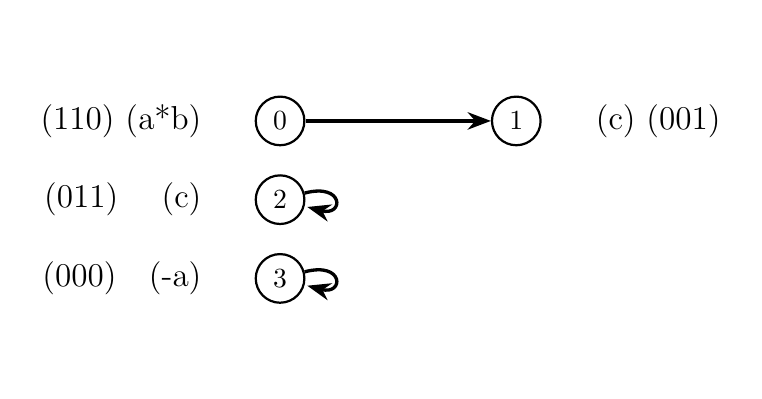
\begin{tikzpicture}
			\begin{scope}[every node/.style={circle,thick,draw}]
			    \node[label={[label distance=0.5cm]180:\large (110)  (a*b)}]  (A) at (0,0) {0};
			    \node[label={[label distance=0.5cm]0:\large (c) (001)}]  (B) at (3,0) {1};
			    \node[label={[label distance=0.5cm]180:\large (011) \ \ \ (c)}]  (C) at (0,-1) {2};
			    \node[label={[label distance=0.5cm]180:\large (000) \ \ (-a)}]  (D) at (0, -2) {3};
			\end{scope}

			\begin{scope}[>={Stealth[black]},
			              every node/.style={fill=white,circle},
			              every edge/.style={draw=black,very thick}]
			    \path [->] (A) edge (B);
			    \path [->] (C) edge[loop right] (C);
			    \path [->] (D) edge[loop right] (D);
			\end{scope}
			\end{tikzpicture}
			\newline
			Let us assume that the variable ids are as:
			\begin{itemize} 
				\item `a` has variable id 0
				\item `b` has variable id 1
				\item `c` has variable id 2
			\end{itemize}
			The bit matrix will be the following:
			\begin{center}
			\begin{tabular}{ |c||c|c|c|c|}
				\hline
				\ & 0 & 1 & 2 & 3 \\
				\hline
				\hline
				0 & 1 & 0 & 0 & 0 \\
				\hline
				1 & 1 & 0 & 1 & 0 \\
				\hline
				2 & 0 & 1 & 1 & 0 \\
				\hline
			\end{tabular}
			\end{center}
			where the rows represent the variable ids, the columns represent the model points.
			The followings are the evaluations of a, b and described in the above matrix,
				namely the evaluation is composed from the positions where there is a one in the column:
			\begin{itemize}
				\item v(a) = \{ 0 \}
				\item v(b) = \{ 0, 2 \}
				\item v(c) = \{ 1, 2 \}
			\end{itemize}

		\paragraph{Contact Matrix} The contact matrix is represented with a contact\_relations\_ variable which type is defined in \ref{sec:contact-matrix}.
			The contact\_relations\_ variable is a symmetric square matrix. The matrix row contact\_relations\_[ i ] gives a bitset of all points which are in contact with the point \textbf{i}. \\
			For example, let us have a model with 6 points:
			\begin{itemize}
				\item[] 0 ---- 1 	\:\:\:\:\:\:, contact between 0 and 1
				\item[] 2 ---- 3 	\:\:\:\:\:\:, contact between 2 and 3
				\item[] 4 		\:\:\:\:\:\:\:\:\:\:\:\:\:\:\:\:\:, point created from $\neq 0$ term
				\item[] 5 		\:\:\:\:\:\:\:\:\:\:\:\:\:\:\:\:\:, point created from $\neq 0$ term
			\end{itemize}

			The contact\_relations\_ will be the following:
			\begin{center}
			\begin{tabular}{ |c||c|c|c|c|c|c|}
				\hline
			        	\ & 0 & 1 & 2 & 3 & 4 & 5 \\
				\hline
				\hline
				0 & 1 & 1 & 0 & 0 & 0 & 0 \\
				\hline
				1 & 1 & 1 & 0 & 0 & 0 & 0 \\
				\hline
				2 & 0 & 0 & 1 & 1 & 0 & 0 \\
				\hline
				3 & 0 & 0 & 1 & 1 & 0 & 0 \\
				\hline
				4 & 0 & 0 & 0 & 0 & 1 & 0 \\
				\hline
				5 & 0 & 0 & 0 & 0 & 0 & 1 \\
				\hline
			\end{tabular}
			\end{center}

		\paragraph{Model Create}
		All models can be created(or at least an attempt can be done for their creation) with the Tableaux branch output \ref{tableaux:branch:output} as its input arguments.
		This is achieved via the 'create' method.
		\begin{lstlisting}
virtual auto create(const formulas_t& contacts_T, 
	const formulas_t& contacts_F, 
	const terms_t& zero_terms_T,
	const terms_t& zero_terms_F, 
	const formulas_t& measured_less_eq_T, 
	const formulas_t& measured_less_eq_F, 
	const variables_mask_t& used_variables, 
	const formula_mgr* mgr)
    -> bool = 0;
		\end{lstlisting}
		
		For simpler explanations in the following algorithms for formula model construction the following constants are introduced. 
		They represent the sizes for the formulas collections which are passed as an argument to the create method of each model construction algorithm.
		\begin{itemize}
			\item N - number of variables in the atomic formulas
			\item M - number of atomic formulas
			\item I - number of Contact atomic formulas
			\item J - number of Non Contact atomic formulas
			\item K - number of Not Equal to Zero atomic formulas
			\item L - number of Equal to Zero atomic formulas
			\item S - number of Measured Not Equal to Zero atomic formulas
			\item U - number of Measured Equal to Zero atomic formulas
		\end{itemize}

		The creation of a model can be done with various algorithms. In this paper the following algorithms will be defined and described in details:
		\begin{itemize} 
			\item Fast Model
			\item Connected Model
			\item Measured Model
		\end{itemize}

	\newpage
		\subsection{Fast Model Algorithm}
			A model is simply a set of points and contacts between them which satisfies the Contacts and Less or equal atomic formulas.

			This model will be easirly explained with an example first:
			\subsubsection*{Example 1.1}
				Let $\varphi$ be the following formula:
				\begin{equation*}
					\varphi = C(a,b) \& C(c,d) \& C(e,f) \& g != 0 \& x = 0 \& ~C(y,z)
				\end{equation*}
				This formula is constructed from 3 contacts, one not equal to zero term, one equal to zero term 
				and one non contact atomic formula.
				\newline
				The model for this formula is constructed from seven modal points, namely two modal points for each
				contact and one point for the not equal to zero term.
				\newline
				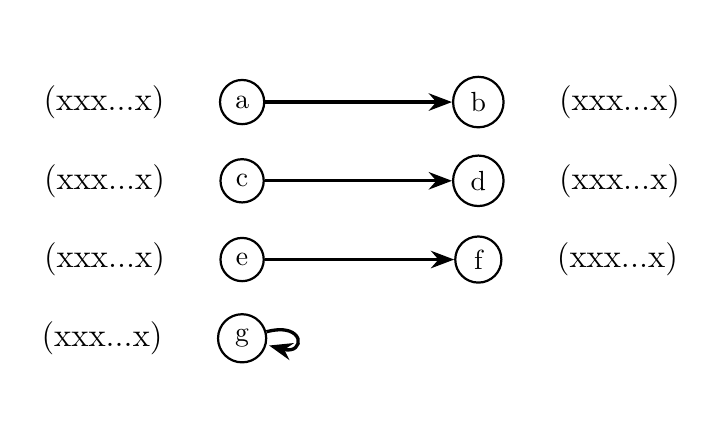
\begin{tikzpicture}
				\begin{scope}[every node/.style={circle,thick,draw}]
				    \node[label={[label distance=0.5cm]180:\large (xxx...x)}]  (A) at (0,0) {a};
				    \node[label={[label distance=0.5cm]0:\large (xxx...x)}]  (B) at (3,0) {b};
				    \node[label={[label distance=0.5cm]180:\large (xxx...x)}]  (C) at (0,-1) {c};
				    \node[label={[label distance=0.5cm]0:\large (xxx...x)}]  (D) at (3, -1) {d};
				    \node[label={[label distance=0.5cm]180:\large (xxx...x)}]  (E) at (0,-2) {e};
				    \node[label={[label distance=0.5cm]0:\large (xxx...x)}]  (F) at (3,-2) {f} ;
				    \node[label={[label distance=0.5cm]180:\large (xxx...x)}]  (G) at (0,-3) {g};
				\end{scope}

				\begin{scope}[>={Stealth[black]},
				              every node/.style={fill=white,circle},
				              every edge/.style={draw=black,very thick}]
				    \path [->] (A) edge (B);
				    \path [->] (C) edge  (D);
				    \path [->] (E) edge (F);
				    \path [->] (G) edge[loop right] (G);
				\end{scope}
				\end{tikzpicture}
				\newline
				In the above graph the (xxx...x) is a bitset, for example (010...1) which gives zero/one evaluation
				for the variables in the formula. Its size is the number of different variables in the formula.
				The model points are the nodes in the graph ranging from 0 to 6. 
				Each node connected to its self, this way the reflexivity of the contacts is represented, and the 
				edges represent the contact relations.
				\newline
				One note can be made that in the above graph the Zero terms and Non Contact atomic formulas are 
				not represented since they do not require existance of model points.

				\subsubsection*{Definition Model Evaluation}
				Model evaluation v which for a given term returns a subset of the model points.
				The model evaluation v is defined as:
				\begin{equation*}
					v(p) = \{ i | (i) (xxx...x)[p] == 1 \} 
				\end{equation*}
				which means that for a given variable p, 
				v(p) returns a set of all points in which the variable p is evaluated to true.

				\subsubsection*{Properties}
				\begin{itemize}
					\item v(a * b) = v(a) \& v(b)
					\item v(a + b) = v(a) | v(b)
					\item v(-a) = ~v(a)
				\end{itemize}

				Note that each point's evaluation evaluates it's term to the constant true in order to that point to be
				in the MODEL evaluation of the term, i.e. for the point 0, 
				the term 'a' and it's evaluation (xxx..x): a->evaluate(xxx..x) = constant\_true 
				in order to 0 belongs to v(a)
				\newline
			
			\subsubsection*{Example 1.2}
				Let $\varphi$ be the following formula:
				\begin{equation*}
					\varphi = C(a,b) \& C(c,d) \& e=0 \& f=0 \& ~C(g,h) \& ~C(i, j)
				\end{equation*}
				Then the model should be of the following type:
				\newline
				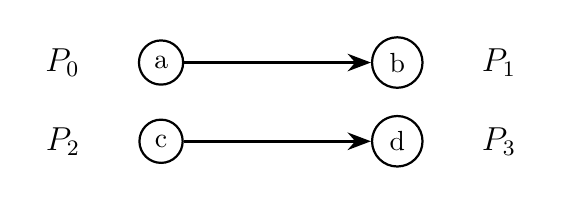
\begin{tikzpicture}
				\begin{scope}[every node/.style={circle,thick,draw}]
				    \node[label={[label distance=0.5cm]180:\large $P_0$}]  (A) at (0,0) {a};
				    \node[label={[label distance=0.5cm]0:\large $P_1$}]  (B) at (3,0) {b};
				    \node[label={[label distance=0.5cm]180:\large $P_2$}]  (C) at (0,-1) {c};
				    \node[label={[label distance=0.5cm]0:\large $P_3$}]  (D) at (3, -1) {d};
				\end{scope}

				\begin{scope}[>={Stealth[black]},
				              every node/.style={fill=white,circle},
				              every edge/.style={draw=black,very thick}]
				    \path [->] (A) edge (B);
				    \path [->] (C) edge  (D);
				\end{scope}
				\end{tikzpicture}
				\newline
				NOTE that if Pi evaluates the term 't' to constant true then the model 
				evaluation v(t) contains the point (Pi \_) (and vice versa)
				\newline
				Where: \\
				P0 evaluates(binary) a to constant true \&\& e and f to constant false \\
			      P1 evaluates(binary) b to constant true \&\& e and f to constant false \\ 
				P2 evaluates(binary) c to constant true \&\& e and f to constant false \\ 
			      P3 evaluates(binary) d to constant true \&\& e and f to constant false \\ 
				Also, to satisfy the requirement for ~C: (we need to check each contact relation): \\
				~[(P0 evaluates g to constant true \&\& P1 evaluates h to constant true) || \\
				(P1 evaluates g to constant true \&\& P0 evaluates h to constant true)] \&\& \\
				~[(P0 evaluates i to constant true \&\& P1 evaluates j to constant true) || \\
				(P1 evaluates i to constant true \&\& P0 evaluates j to constant true)] \&\& ... analogous for P2 and P3. \\
				\newline
				The contact relation is reflexive, so for each point we also need to check also:	\\
				~(Pi evaluates g to constant true \&\& Pi evaluates h to constant true) \&\& \\
				~(Pi evaluates i to constant true \&\& Pi evaluates j to constant true)

			\paragraph{Algorithm}
			% NOTE Intro on what the fast model really is !
			Let us have $\varphi$ in the format defined in the definition of \hyperref[tableaux:branch:output]{the tableaux branch output}. % for now this is formula 4 
			Let us define few constants which will ease the annotation:
			\begin{itemize}
				\item N - number of variables in the atomic formulas
				\item M - number of atomic formulas
				\item I - number of Contact atomic formulas
				\item J - number of Non Contact atomic formulas
				\item K - number of Not Equal to Zero atomic formulas
				\item L - number of Equal to Zero atomic formulas
			\end{itemize}
			
			Note: The term evaluation is with an accumulated complexity of O(L) which is not included in the O notation bellow.
			\newline
			\newline
			The algorithm which creates such points in an iterative manner is as follows:
			\newline
			1) Creates contact points, i.e. for each C(a,b) we create two points Pa and Pb.  \\
				Note that a point is just an variable evaluation. \\
				They satsfy the following rules: 
				\begin{itemize}
					\item Pa[a]=1 and Pb[b]=1.
					\item does not break any t=0 atomic formula, \\
						i.e. Pa[t]=0 and Pb[t]=0.
					\item does not break the reflexivity part of all ~C(e,f) atomic formulas, \\
						i.e. Pa[e]=0 \& Pa[f]=0 \& Pb[e]=0 \& Pb[f]=0.
					\item does not break any ~C(e,f) atomic formulas, \\
						i.e. ~[(Pa[e]=1 \& Pb[f]=1) | (Pb[e]=1 \& Pa[f]=1)]
				\end{itemize}
				
				If any of the rules above is not satisfied we change Pb's evaluation, 
				if not possible to generate a new evaluation for Pb then we change 
				Pa's evaluation and reset the Pb's evaluatuion to the 'first' one.

				If again some rules is broken we change Pb's evaluation, etc. 
				if we can't generate new evaluation for Pa then there is no satisfiable model.
				\newline

				Complexity for this step: O(2\^N * 2\^N * (G+M))
				\newline
				\newline
				2) Creates a point for each a!=0 atomic formula - Pa, which satisfy the following rules:
				\begin{itemize}
					\item Pa[a] = 1
					\item does not break any t=0 atomic formula, \\
						i.e. Pa[t]=0
					\item does not break the reflexivity part of all ~C(e,f) atomic formulas, \\
						i.e. Pa[e]=0 \& Pa[f]=0
				\end{itemize}

				If any of the rules above is not satsfied with Pa, 
				then we generate next Pa's evaluation and check them again. 
				If not possible to generate next evaluation then there is no satisfiable model.
				\newline

				Complexity for this step: $O(2^N * (G+M))$
				\newline
				\newline
				3) We create the contact connectivity matrix - 
				PxP in a simple way because we know that only first 2K points are in contact.
				0 <= i < K: set a contact relation between point i and i+1, 
				i.e. we set the bit [i][i+1] to 1 and [i+1][i] to 1.
				\newline

				Complexity for this step: $O(P^2)$
				\newline
				\newline
				5) We calculate the v(X) for each variable.
				We create a vector of N bitsets. 
				Each bitset will hold all points in the evaluation of that variable, 
				i.e. bitset at position 'j' is the set v(j), where 'j' is some variable id.
				\newline

				For each point Pi, we iterate over the set bits in it's evaluation and 
				if we have a set bit at position j we add that point to the evaluation 
				of varialbe 'j', i.e. we set the bit 'i' in the variable's evaluation bitset.
				\newline

				Complexity for this step: O(P * N)
				\newline
				\newline

				Overall Complexity: $O(2^N * 2^N * (G+M))$
					% (I suppose that 2^N >>> P)

	\newpage
	\subsection{Connected Model}
		A Connected model is called a formula model for which the following lemma is true.
		\subsubsection*{Connectivity Lemma}
		\begin{equation}
			\forall a \in R: a \neq \emptyset \vee a \neq \mathbb{W} \leftarrow C(a, \overline{a})
		\end{equation}
		\paragraph{Connected Model Algorithm}
		Let $\varphi$ be the input formula, on which the tableaux process is applied, thus returning the tableaux branch output \ref{tableaux:branch:output}.
		1) Let $\mathbb{M}$ denote the model of all possible unique model points, where one model point corresponds to 
			one variable evaluation $P_i$. 
			\newline
			Since there are N variables, the number of unique model points is $2^N$.
			\newline

			1.1) Filter out the model points which interfere with the zero terms, 
			which means that if $P_i$ evaluates some term $G_l$ to constant true then $P_i$ is filtered out.
			\newline

			1.2) Filter out the model points which interfere with the Non contants, which mens that 
				If $P_i$ evaluates some terms $E_j$ and $F_j$ to true, then $P_i$ is filtered out.
			\newline

			NOTE: that if $P_i$ evaluates the term $\tau$ to constant true then the model 
			evaluation v($\tau$) contains the point $P_i$ (and vice versa).
			\newline
			\newline
		So far, the model $\mathbb{M}$ satisfies all Equal to Zero atomic formulas and 
		the reflexivity property of the Non Contacts.
		\newline TODO: explain reflexivity of contacts in the theoretical part.
			\newline
			\newline		
		2) Verification is done for the Not Equal to Zero atomic formulas in $\mathbb{M}$, namely:
			\begin{equation}
				\text{If  } \exists k: v(D_k) \neq \emptyset \text{ , then there does not exist a connected model.}
			\end{equation}

		2.1) Verification is done for the Contact atomic formulas in $\mathbb{M}$, namely:
			\begin{equation}
				\text{If  } \exists i: v(A_i) = \emptyset \vee v(B_i) = \emptyset \text{, then there does not exist a connected model.}
			\end{equation}
			\newline
		So far, $O(2^N * N)$ bits of memory to hold all points and 
		their evaluations and $O(2^N * M)$ time to process them.
			\newline
			\newline	
		3) Let $\mathbb{C}$ be a bit matrix of size $2^N x 2^N$.
			\newline
			
			This matrix will be called connectivity matrix and will represent the connected points in $\mathbb{M}$.
			
			\begin{equation}
				\text{Model points i and j are in contanct if } \mathbb{C}[ i ][ j ] \text{ is set.}
			\end{equation}

			Initialy all points are in contact, which means that the initial value of each bit is set:
			\begin{equation}
				\text{Let } \forall i, j < 2^N : \mathbb{C}[ i ][ j ] = 1
			\end{equation}
	
			3.1) Remove all connections which interfere with Non Contact atomic formulas.
				\begin{align*}
					\forall a, b < 2^N, \forall j < J :& \\
						\text{if } P_a [E_j] = 1 \wedge P_b [F_j] = 1 &\vee P_a[F_j] = 1 \wedge P_b[E_j] = 1, \\
						\text{then unset } \mathbb{C}[a][b] &\text{ and } \mathbb{C}[b][a].
				\end{align*} 
				
			Note that the reflexivity has been satisfied in 1).
			\newline

			For this step $O(2^N * 2^N) = O(2^{2*N})$ bits of memory were used and 

			total of $O(2^N * 2^N * J)$ time complexity.
			\newline
			\newline	
		4) Check that all Contacts are still satisfied
			\begin{equation}
				\forall i, j < 2^N: C(A_i, B_i) \text{ is satisfied}
			\end{equation}
			
			The check whether $C(A_i, B_i)$ is satisfied is done in the following maner:
			
			\begin{equation}
				\forall p \in v(A_i): (\mathbb{C}[p] \text{  bit\&  } v(B_i)) \neq 0
			\end{equation}
			Where $\mathbb{C}[p]$ is a bitset representing all contacts of p and 
			$v(B_i)$ is a bitset representing the evaluation of $B_i$.
			\newline
			Thus $(\mathbb{C}[p] \text{  bit\&  } v(B_i)) \neq 0$ means that there is 
			a common point between the evaluation of $B_i$ and the contacts of p.
			\newline
			\newline
			The complexity for this step is: $O(I * (H + L * G)$,where: 
			\begin{itemize}
				\item H is the complexity for evaluation some term, 
					it's at most the number of operations in the term, something small.
				\item L is the number of points in $v(A_i)$ which is at most $2^N$.
			       \item G is the complexity for "bit operator \&" which is $2^N/2^6$.
			\end{itemize}
		5) The previous step produces the maximal unique satisfiable model, wihch is a graph $\mathbb{G}$.
			If there exists a satisfiable connected subgraph in the $\mathbb{G}$, then this is the connected model.
			Finding all connected subgraphs has time complexity of $O(2^N + 2^N * 2^N)$.
			Checking if a subset of points satisfies the formula can be done in a similar fashion(as the one above).
			\newline
			Note that only the check for Not Equal to Zero and Contacts atomic formulas has to be done, 
			since when a point is removed the  Equal to Zero and Non Contacts atomic formulas can not be broken.
			\newline
			Let Y be the number of points in the subset, then at most $O(Y * Y * M)$ time complexity.
			Note that this must be done for ach connected subgraph and the subgraphs are not overlapping!
			Upper bound for Y is $2^N$, so the upper bound and on the time complexity is: 
			\begin{equation*}
				O(2^N * 2^N * M),
			\end{equation*}
			since 
			\begin{equation*}
				x * x * M + y * y * M <<< (x+y)*(x+y)*M
			\end{equation*}
			\newline
			\newline	
		Overall memory complexity: $O(2^N * 2^N)$ bits
		\newline
		Overall time complexity: $O(2^N * 2^N * M)$

	\newpage
	\subsection{System of Inequalities}
		The systems are of the following type:	
		\[
			\syslineskipcoeff{1.50}
			\systeme*{\sum_{i^1} X_{i^1} <= \sum_{j^1} X_{j^1},
				\:\:.\:\:.\:\:.,
				\sum_{i^n} X_{i^n} <= \sum_{j^n} X_{j^n}, 
				\sum_{k^1} X_{k^1} > \sum_{l^1} X_{l^1},
				\:\:.\:\:.\:\:.,
				\sum_{k^m} X_{k^m} > \sum_{l^m} X_{l^m}
				}
		\]
	
		To calculate these systems of inequalities a third party library is used, which is specialized 
		to solve systems of inequalities. The library's name is Kiwi.
		\newline
		\subsection{System Construction}
		The system of inequalities is constructed from the potential meassured model by evaluating each
		of the terms in the Meassured less or equals and Meassured greater atomic formulas. The points in the model are 
		enumerated from 0 to N - 1, where N is the number of model points. The system will have N different variables $X_0, X_1, ..., X_n$, 
		where $\forall i < N: X_i \text{ is mapped to point i}$
		\newline
		TODO: Add beter theoretical explanation
		\newline
		\newline
		1) For each <=m(x, y) calculate v(x) and v(y), then an inequality of the following type is created: 
		\begin{align*}
			\sum_{i \in v(x)} X_i <= \sum_{j \in v(y)} X_j
		\end{align*}

		If some X is on both sides of an inequality, then both of them are removed.
		\newline
		2) For each \textasciitilde<=m(x,y) calculate v(x) and v(y), then an inequality of the following type is created: 
		\begin{align*}
			\sum_{i \in v(x)} X_i > \sum_{j \in v(y)} X_j
		\end{align*}

		If some X is on both sides of an inequality, then both of them are removed.
		\newline

		3) For each variable in the model a new greater than constraint is added to the system
		\newline
		If the system of inequalities constructed in this maner has solution, then this system of inequalities
		satisfies the meassured model.

		\subsection{Meassured Less Operator Representation}
		All of the researched third party libraries for solving systems of inequalities work only with Less or Equal inequalities.
		This means that the greater inequalites must be simulated with the usage of Less or Equal inequalities.
		\newline
		This absence is solved with the addition of a really small variable while converting the greater inequality to 
		less or equal inequality.
		\newline
		Let us have the following inequality
		\[
			\syslineskipcoeff{1.50}
			\systeme*{\sum_{i^1} X_{i^1} > \sum_{j^1} X_{j^1}}
		\]
		then this inequality is transformed into:
		\[
			\syslineskipcoeff{1.50}
			\systeme*{0 <= \sum_{i^1} X_{i^1} - \sum_{j^1} X_{j^1}} + \epsilon
		\]
		where $\epsilon$ is a small value.
		\newline
		The inequality X > 0, which is a variable to be greater than zero is transformed into:
		\[
			\syslineskipcoeff{1.50}
			\systeme*{0 <= X - \epsilon} 
		\]
		\newline
		Google's linear solver Glop (OR-Tools) was one of the tested libraries and it has precision around $1*10^{-7}$.
		Kiwi's precision is around $1*10^{-8}$. 
		\newline
		These results are based on simple empirical testing, namely:

		A simple system of only one inequality $X > 0$ which is converted to $X - \epsilon >= 0$. 
		While testing the $\epsilon$ value was slowly decreasing and when it gets smaller than $1*10^{-7}$
		($1*10^{-6}$ for google's Glop (OR-Tools) ) the solver gave a wrong answer.
		\newline
		\newline
		Besides this anomaly, the precision is good enough for the purposes of finding solutions for the special type
		of systems of inequalities defined above.

	\newpage
	\subsection{Measured Model}
		% NOTE Intro on what the measured model really is !
		Let us have $\varphi$ in the format defined in the definition of \hyperref[tableaux:branch:output]{the tableaux branch output}. % for now this is formula 4 
		
		\subsubsection*{Points construction}
		The Measured Model is composed of modal points, the number of modal points is $I + L + S + U$.
		
		The following atomic formulas produce an existance of a modal point:
		\begin{itemize}
			\item $C(A_i, B_i)$ produces two modal points, \\
				where x and y are terms.
			\item $g_l \neq 0$ produces one modal point, \\
				where x is a term.
			\item $<=_m(H_s, O_s)$ produces one modal point
			\item $\neg (<=_m(Q_u, R_u) )$ produces one modal point
		\end{itemize}
		For each contact $C(A_i, B_i)$ two new model points are created A and B, where $A \in v(A_i) \text{ and } B \in v(B_i)$.
		In some cases the point created for a contact might be one, but this in turn is simulated by having the same evaluation for two 
		points, which means that the point is duplicated.
		\newline
		Each Point will be represented with $P(\tau , e)$, where $\tau$ is a term and e is the variable evaluation.
		The point's evaluation P[e] positively evaluates the point's term $P[\tau ]$, meaning that P belongs to $v(P[\tau ])$.
		\newline
		Example: Let's have C(a + b, c*d)
		\newline
		then a valid model point for 'a + b' is P('a+b', [1000]), where [1000] is the evaluation for (a, b, c, d) variables.
		That evaluation evaluates 'a+b' to true.
		\newline
		For 'c*d' a point could be: P('c*d', [0011]).
		\newline
		All possible combinations of such points are $2^{N * (I + L + S + U)}$, since there are $I + L + S + U$ number of points and 
		each point has $2^N$ potential evaluations.
		\newline
		The following algorithm determins if there is a satisfiable measured model.

		\subsubsection*{Measured Model Algorithm}

			1)  For each $C(A_i, B_i)$ two points are created $P_a$ and $P_b$: $P_a[A_i] = true$ and $P_b[B_i] = true$.
				If not possible - then there is no satisfiable model.
			\newline
			\newline
			2) For each $g_l \neq 0$ one point is created P: $P[g_l] = true$.
				If not possible - then there is no satisfiable model.
			\newline
			\newline
			3) For each measured atomic formula a modal point is created which is associated to '1' constant term.
			\newline
			\newline
			4) A connection is made between the contact points, first 2*I points are from Contact terms,
				 i.e. for each 0 <= i < I a connection is added in the connectivity matrix between 2*i and 2*i + 1 points. % NOTE DEF CONNECTIVITY MATRIX
			\newline
			
			A new combination of points is generated by 9) until the steps from 5 to 8 are satisfied.
			\newline

			5) Calculate the v(X) for each variable. % (TODO: this should be explained somewhere else already)
			\newline

			6) For each $G_l \neq 0$ evaluate $v(G_l)$ and check that it is not the empty set. O(L)
			\newline

			7) For each \textasciitilde $C(E_j, F_j)$ check that $v(E_j)$ and $v(F_j)$ does not contain a common point and that $v(E_j)$ does not contain a point which is in contact with a point $v(F_j)$.
			\newline

			Complexity: O(J * (I + J) * G)
			\begin{itemize}
				\item G is the complexity for "bit operator \&" which is something like $(I+J)/2^6$.
				\item I+J is the number of points.
			\end{itemize}
			
			8) Check the measured atomics: \\% TODO: we should have already defined why we are doing it in some theoretical part of the documentation 

			For each $<=_m(H_s, O_s)$ calculate $v(H_s)$ and $v(O_s)$ and create an inequality of the following type: 
			\begin{align*}
				\sum_{i \in v(H_s)} X_i <= \sum_{j \in v(O_s)} X_j
			\end{align*}
			For each $\neg (<=_m(Q_u, R_u) )$ calculate $v(Q_u)$ and $v(R_u)$, create an inequality of the following type: 
			\begin{align*}
				\sum_{i \in v(Q_u)} X_i > \sum_{j \in v(R_u)} X_j
			\end{align*}
			Each inequality is a row in the system of inequalities. 
			If this system has a solution, then the generated model is a satisfiable one. \\ % say that the above def of system of in. is the solver
			
			Finish!
			\newline

			9) The generation of new combination of points: \\
				Similar to binary +1 operation but instead of just 0 and 1 states on each position there are $2^N$ combinations,
				from which some will not be valid because they will not evaluate the point's term to true
			\newline
			Here is an example of binary +1 operation:
			\begin{align*}
				000 + 1 &= 001 \\
				001 + 1 &= 010 \\
				010 + 1 &= 011 \\ 
				011 + 1 &= 100 \\
				100 + 1 &= 101 \\
				101 + 1 &= ...
			\end{align*}
			If there are two variables and two points and for the sake of simplicity ignore the term for now.
    			At first there will be only 0s. \\
			$[00][00]$ where the first [00] is the evaluation of the first point which evaluates both variables to 0.
			\newline
			The next generations looks as follows:
			\begin{align*}
				[00][00] -(&\text{next combination})-> [00][01] \\
				->& [00][10] \\
				->& [00][11] \\
				->& [01][00] \\
				->& [01][01] \\
				->& [01][11] \\
				->& [10][00] \\
				-..->& [11][11]
			\end{align*}
			In the above example the [11][11] is the last combination.
			\newline
    			When the condition that the point's evaluation should evaluate the term to true is taken into account, then all evaluation which do not evaluate the 
			term to true are skipped.
			\newline
    			Example: if the variables are 'x' and 'y', first point's term is 'x', second point's term is 'y' then the valid sequence of combinations will be:
			\begin{align*}
				[x:1 y:0, 'x']&[x:0 y:1, 'y'] -> [10][11]  \\
				->& [11][01] \\
				->& [11][11]
			\end{align*} % WHAT ? 
			\newline

			TODO: THIS complexity should be explained and recalculated:
			\newline
			Complexity: O((I + L + S + U) * G), where G is the complexity for finding a next evaluation for a point, 
			namely finding an evaluation which evaluates the point's term to true.

	\newpage
	\section{Rest Server}
		The Web Server is used to serve:
		\begin{itemize}
			\item Rest APIs
			\item Resources
		\end{itemize}
		The Rest APIs are used to chek for satisfiability, to find connected models or meassured models.
		\newline
		The resources are:
		\begin{itemize}
			\item Html pages
			\item Images 
			\item Javascript code
			\item Styles
		\end{itemize}
		The Web Interface is easy to use, contains only the needed information and from there 
		can be executed all of the described satisfiability algorithms.

		One client can execute only one algorithmic program at a time. 
		This way it is ensured that there are not a lot of simultaneous executing programs by the server.
		
		If the program execution time gets too long the client has the possibility to terminate the execution 
		of the current program by server. This will re-enable the client to execute another program and will remove 
		the execution load from the server.

		If the client posts a couple formula for calculation and terminetes the session (for example closes the browser),
		then the task in the backend will be terminated as well.

		\subsection*{Output}
		The output of the program is separated in three modules:
		\begin{itemize}
			\item Resulting output - indicates what was the final result of the execution. \\
				For example: The formula is satisfiable.
			\item Verbose output - This is the output which contains the full proof of the formula execution. \\
				This output is printed though the whole execution.
			\item Visualized graph - This is the end result of the model, if such model exists \\
				The visualization is done with a JavaScript third party library for drawing graphs.
		\end{itemize}
	\newpage
	\begin{thebibliography}{9}
	\bibitem{flex-tokenizer} 
		Flex Tokenizer,
		\\\texttt{http://web.mit.edu/gnu/doc/html/flex\_1.html}

	\bibitem{bison-parser} 
		Bison Parser,
		\\\texttt{https://www.gnu.org/software/bison/}

	\bibitem{visitor-pattern} 
		Visitor Pattern,
		\\\texttt{https://en.wikipedia.org/wiki/Visitor\_pattern}
	\end{thebibliography}
\end{document}










































